% !TEX root = main.tex
\documentclass[a4paper, UKenglish, 11pt]{uiomaster}
\usepackage{lipsum}
\usepackage[subpreambles=true]{standalone}
\usepackage[table,xcdraw]{xcolor}
\usepackage{hyperref}
\usepackage{xcolor}

\begin{document}

\chapter{Extending the DiLoc Network}
Until now we have seen how DiLoc as a feed forward neural network and a compatible CNN shows satisfying predictions in localizing single and multipole current dipoles. In this chapter we will build upon the DiLoc network, modifying it to not only find the position of dipoles, but the characteristics of magnitude of dipole signal and radius of larger populations of dipoles. We explore a set of extensions and small modifications to the DiLoc network aimed at enhancing its capability to identify characteristics of current dipoles besides also addressing the inverse problem. We delve into two distinct extensions of the initial inverse problem, challenging DiLoc's predictive capabilities in handling more complex scenarios.

The first case involves extending the dataset by assigning individual magnitudes to each dipole source. This extension presents the network with the task of predicting both location of the source and its corresponding magnitude. Subsequently, the second scenario transitions from predicting the location of a single dipole source to estimating the center and radius of a population of dipoles, alongside the magnitude of the electrical signals generated. This extension introduces additional complexities to the localization process.

\section{Method: Adjusting Data Set and Architecture}
Throughout the chapter, we methodically introduce distinct modifications to DiLoc for each problem, assess the network's performance, and offer insights into its strengths and limitations when addressing these novel challenges. However, before delving into the results, we will first address important considerations that apply to both extensions. This encompasses ensuring DiLoc effectively handles varying units in its output, selecting an optimal cost function tailored to our specific problems, and establishing criteria for assessing DiLoc's performance in the context of its intended tasks.

\subsection{Scaling of Target Values}
In addressing the extended problems within DiLoc, the network is tasked with predicting target values with significant variations in both range and units. This necessitates an essential preprocessing step: the scaling of target data. The importance of this scaling stems from the fact that the traditional cost function calculates differences between predicted output and actual target values, and add together the distinct terms within the loss. When the target values exhibit disparities in their ranges and units, several challenges arise.

Firstly, it is imperative to acknowledge that attempting to aggregate \rednote{add together} losses from distinct target values with varying units lacks a straightforward and intuitive approach. Combining values with different units into a single loss function can lead to an ambiguous interpretation and hinder the meaningful evaluation of the network's performance.

Secondly, the variation in the range of target values poses a potential issue. Variations can result in certain dimensions being imbalanced in their influence on the overall error, potentially overshadowing dimensions with smaller ranges. This asymmetry in the error calculation can lead to a biased optimization process and hinder the network's ability to effectively learn from the data.

To mitigate these challenges, we employ a normalization technique that transforms the output values into a consistent range, specifically ranging from 0 to 1. This normalization is achieved using the following formula:

\begin{equation}
\tilde{y_i} = \frac{\tilde{x_i} - \tilde{\text{min}(x)}}{\tilde{\text{max}(x)} - \tilde{\text{min}(x)}}
\label{eq:scale_target}
\end{equation}

Here, $\tilde{y_i}$ represents the i$^{\text{th}}$ normalized value in the dataset for a specific target category, $x_i$ is the i$^{\text{th}}$ value in the corresponding target dataset, and min($x$) and max($x$) denote the minimum and maximum target values for the specific target category.

It is essential to emphasize that this normalization process is performed separately for each target category. By normalizing the target values in this manner, we strive to create a more equitable cost function where all target values contribute equally to the overall error calculation. Consequently, DiLoc can harness its learning capabilities more effectively and hopefully perform better in its tasks.



\subsection{Sigmoid as Last Layer Activation Function}
In the problem concerned with predicting the postion of a single dipole source, DiLoc did not have any activation function in the last layer.
However, considering that the output data has been normalized to a range from 0 to 1, we deem it appropriate to employ the \emph{Sigmoid} activation function in the output layer.

The Sigmoid function is known as one of the more biologically plausible activation functions as the ouput of inactivated neurons returns zero \cite{Jensen2022}. More precised it is a logistic mathematic function meaning that it maps its input to a value between 0 and 1:

\begin{equation}
  f(x) = \frac{1}{1 + e^{-x}}
\label{eq:Sigmoid}
\end{equation}

The Sigmoid function maps the output values to a range between 0 and 1, which aligns with our desired output range, for the exteded problems. This choice of last layer output function may potentially facilitate the training process, as it enables the network to converge more effectively towards the desired outputs, and resticts the network from outputting values outside the desired rarget range.

\begin{figure}
    \centering
    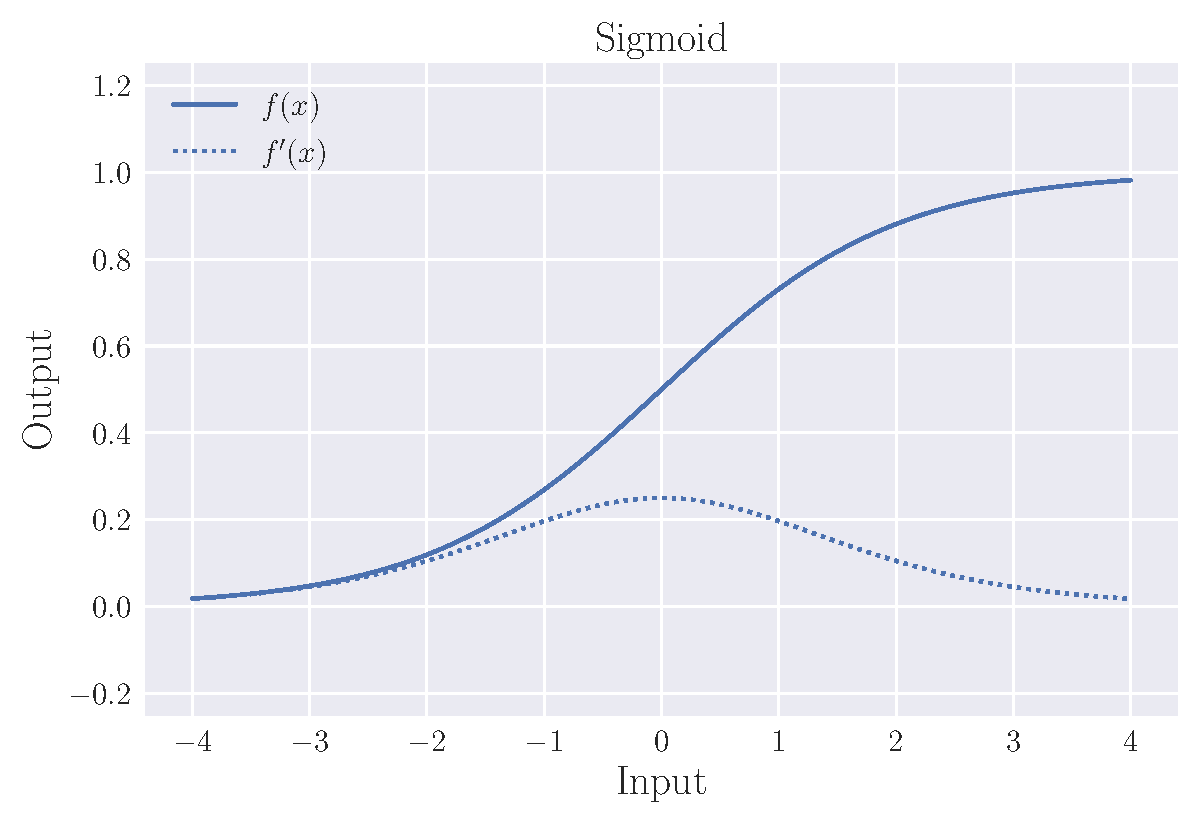
\includegraphics[width=\linewidth]{figures/Sigmoid.pdf}
    \caption{\rednote{Need cite and figure text.} Sigmoid activation function.}
    \label{fig:sigmoid}
\end{figure}


\subsection{Choosing an Optimal Cost Function}
% Include data distribution (min/max)
Selecting an appropriate cost function for is pivotal in addressing machine learning challenges. In regression tasks like ours, the mean squared error (MSE) is a widely used cost function, particularly suitable for linear regression. The MSE is preferred due to its simplicity and continuous measure of model performance during training. It calculates the squared differences between the model's predictions and target values, then takes the mean across the entire dataset.

Having a clear understanding of our desired model outcomes, we aim to develop a customized cost function that aligns precisely with our specific objectives. This tailored cost function may potentially outperform the Mean Squared Error (MSE) cost function, which we previously utilized.

Our new objective is to create a model capable of accurately predicting not only the positions of individual dipoles but also various aspects of dipole signals, including their magnitudes, the radii of extended dipole populations, and the positions of dipole pairs where both contribute to the complete EEG signal.

To achieve this objective, our ideal cost function is composed of several components. Firstly, it should minimize the Euclidean distance between target dipole localizations ${\theta}{x,y,z}$ and their true values $\tilde{\theta}{x,y,z}$:

\begin{equation}
    \text{MED}_{x,y,z}(\boldsymbol{\theta}) = \frac{1}{n}\sum_{i=0}^{n-1}\sqrt{(\theta_{x,i} - \tilde{\theta}_{x,i})^2 + (\theta_{y,i} - \tilde{\theta}_{y,i})^2 + (\theta_{z,i} - \tilde{\theta}_{z,i})^2},
\label{eq:MED}
\end{equation}

Additionally, the cost function should minimize the absolute error between the predicted magnitude ${\theta}{A}$ and the true magnitude $\tilde{\theta}{A}$:

\begin{equation}
    \text{MAE}_{A}(\boldsymbol{\theta}) = \frac{1}{n} \sum_{i=0}^{n-1} \| \theta_{A,i} - \tilde{\theta}_{A,i} \|,
\label{eq:MAE_A}
\end{equation}

Similarly, it should minimize the error between the predicted radius ${\theta}{\text{r}}$ and the true radius $\tilde{\theta}{\text{r}}$:

\begin{equation}
    \text{MAE}_{r}(\boldsymbol{\theta}) = \frac{1}{n} \sum_{i=0}^{n-1} \| \theta_{r,i} - \tilde{\theta}_{r,i} \|,
\label{eq:MAE_r}
\end{equation}

Finally, the cost function should minimize the Euclidean distance among a set of $m$ dipoles in the $x-$, $y-$ and $z-$ dimensions. This is expressed by the equation:

\begin{equation}
\begin{aligned}
    \text{MED}_{x_1, y_1, z_1,\ldots, x_m, y_m, z_m}(\boldsymbol{\theta}) = \frac{1}{n}\sum_{i=0}^{n-1}&\Biggl( \sqrt{(\theta_{x_1,i} - \tilde{\theta}_{x_1,i})^2 + (\theta_{y_1,i} - \tilde{\theta}_{y_1,i})^2 + (\theta_{z_1,i} - \tilde{\theta}_{z_1,i})^2} \\
    & + \quad \sqrt{(\theta_{x_2,i} - \tilde{\theta}_{x_2,i})^2 + (\theta_{y_2,i} - \tilde{\theta}_{y_2,i})^2 + (\theta_{z_2,i} - \tilde{\theta}_{z_2,i})^2}
   \\ & + \quad \ldots \\
    & + \quad \sqrt{(\theta_{x_m,i} - \tilde{\theta}_{x_m,i})^2 + (\theta_{y_m,i} - \tilde{\theta}_{y_m,i})^2 + (\theta_{z_m,i} - \tilde{\theta}_{z_m,i})^2} \Biggr)
\end{aligned}
\label{eq:MED_multiple_dipoles}
\end{equation}

We note, that in the context of our problem involving multiple dipoles, the target vector comprises two sets of coordinates corresponding to the positions of the dipoles we aim to predict. Similarly, the output vector contains two sets of coordinates. Traditional cost functions, such as Mean Squared Error (MSE), straightforwardly map the first set of coordinate vectors in the target with the first set of coordinates in the output, assuming that the order is correct and that every element should align perfectly. However, this approach can overlook the possibility that another permutation could represent the correct mapping.

Our network's primary task is to decipher patterns and learn from EEG data. It may not inherently grasp the correct order in which to place the coordinates of two dipoles (i.e., which should come first or second in the output vector), potentially leading to suboptimal mappings that misguide the network's weight updates during loss calculation. This limitation could increase computational time or, in the worst case, hinder the network's learning process.

To overcome this challenge, our customized cost function systematically explores all possible permutations of target and output vectors, ensuring that the network explores all valid combinations and determine which combination yields the minimum loss. Once we identify the optimal permutation, we use it to calculate the cost using the equation above \ref{eq:MED_multiple_dipoles}. This approach fosters more effective learning and adaptation to various scenarios, enabling the network to capture the genuine underlying patterns in the data. By enabling the cost function to compute all permutations and select the one yielding the minimum loss, we provide the network with the necessary flexibility to excel in this complex task.

\rednote{Add where unit tests can be found?}
For all terms within the cost function, comprehensive unit tests have been developed to confirm its intended functionality. Each problem introduced for the network corresponds to a distinct form of the customized cost function:

\begin{equation}
    C(\boldsymbol{\theta}) =
    \begin{cases}
      \begin{array}{l}
      \text{MED}_{\text{x,y,z}}(\boldsymbol{\theta}),
      \end{array} & \text{if } \| \boldsymbol{\theta} \| = 3\\
      \\
      \begin{array}{l}
      \text{MED}_{\text{x,y,z}}(\boldsymbol{\theta}) + MAE_{\text{A}}(\boldsymbol{\theta}),
      \end{array} & \text{if } \| \boldsymbol{\theta} \| = 4\\
      \\
      \begin{array}{l}
      \text{MED}_{\text{x,y,z}}(\boldsymbol{\theta}) + MAE_{\text{A}}(\boldsymbol{\theta}) + MAE_{\text{r}}(\boldsymbol{\theta}),
      \end{array} & \text{if } \| \boldsymbol{\theta} \| = 5\\
      \\
      \text{MED}_{\text{x}_1,\text{y}_1,\text{z}_1,\ldots,\text{x}_m,\text{y}_m,\text{z}_m}(\boldsymbol{\theta}), & \text{otherwise}
    \end{cases}
    \label{eq:cost_function}
\end{equation}

Here, $| \boldsymbol{\theta} |$ signifies the length of the target vector. When $| \boldsymbol{\theta} | = 3$, the simplest problem is considered, where the network predicts the coordinates of a single-point current dipole, as explored in the previous chapter(s). If $| \boldsymbol{\theta} | = 4$, the network predicts the $x$-, $y$-, and $z$-coordinates of a single dipole, in addition to the magnitude of the signal strength. When $| \boldsymbol{\theta} | = 5$, the target vector encompasses all previously mentioned values, along with the size of a current dipole population with radius. Finally, for $| \boldsymbol{\theta} |$ greater than 5, the multiple dipole problem is addressed, where the network predicts the locations for two or more point source dipoles situated at distinct positions within the cortex.

\rednote{IMPORTANT: This need modifications!}
In crafting our customized cost function, it is important to acknowledge that, like the built-in Mean Squared Error (MSE) cost function, our formulation inherently treats all target values equally during the optimization process. In other words, the algorithm assigns the same weight to each target value when striving to reduce the overall loss. This approach ensures that errors of equal percentage magnitude in different target values are treated on a level playing field. Consequently, a 1$\%$ error for one target value is considered as important as a 1$\%$ error for another target value, regardless of the specific range or scale of these values.

It is worth noting that our choice to uniformly weight all target values is an intentional design decision. While alternative approaches, such as assigning different weights to different target values, could have been explored, we prioritize the creation of a balanced model that can accurately predict all facets of our target values. This approach stems from our objective of achieving a comprehensive understanding of EEG signal sources through a holistic and equitable modeling approach.

Moreover, this uniform weighting approach aligns with our broader modeling philosophy, emphasizing the creation of a model that is versatile and adaptable across a spectrum of EEG data variations. Our aim is not only to develop a model capable of accurately predicting target values but also to ensure that its predictive capabilities are unbiased and comprehensive, covering the multifaceted aspects of EEG signal analysis.

In this way, our customized cost function showcases the fusion of machine learning principles with the nuanced requirements of clinical medicine, as we strive to bridge the gap between technical prowess and real-world medical applications.


\subsection{Overview on Arcitecture and Hyperparameters}
In figure \ref{fig:NN_dipole_w_amplitude_architecture} we have illustraded the architecte of the extended DiLoc network, outputting $m$ target values, depending on the problem to solve. We see that DiLoc still takes an input of 231 data points corresponding to the number of recoring electrodes, and still has the same number of layers and nodes in each layes, except from the output layer.

\begin{figure}[!htb]
    \centering
    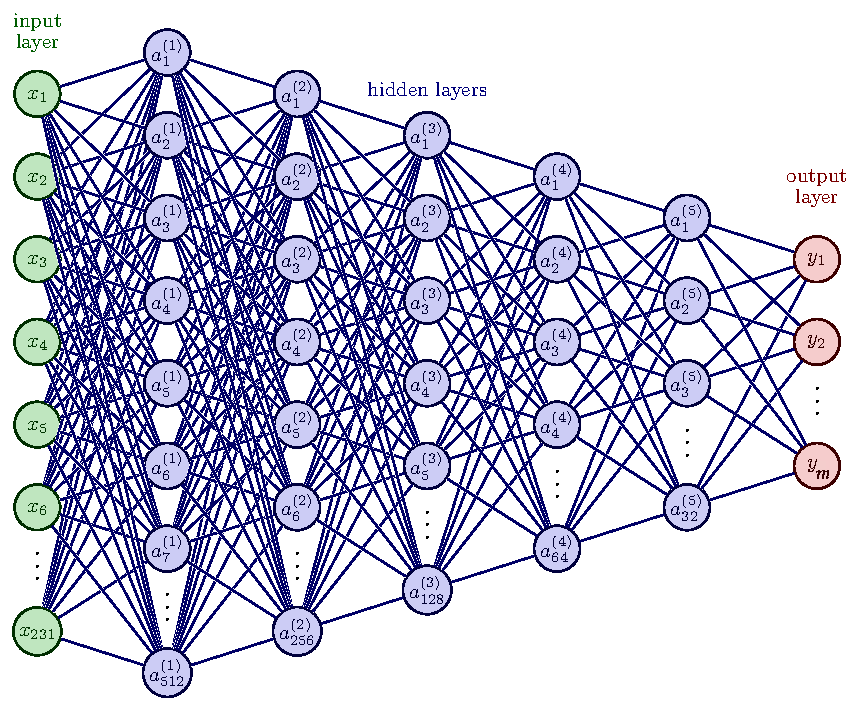
\includegraphics[width=\linewidth]{figures/NN_architecture_multiple_outputs.pdf}
    \caption{Architecture dipole with amplitude.}
    \label{fig:NN_dipole_w_amplitude_architecture}
\end{figure}

% Is it true that sigmoid helpt the efficentcy of the lerning process for the network? For improvements, it would be beneficial to elaborate on the rationale behind using hyperbolic tangent for the hidden layers and ReLU for the first layer.
In the extension of the DiLoc network, we maintain the use of ReLU as the activation function in the first layer, and hyperbolic tangent for the hidden layers, as this architecture, combined with the chosen hyperparameter for all problems considered gave the most promising results. However, as explained above, we deem it appropriate to employ the Sigmoid activation function in the output layer.

For an overview of the overall parameters employed in the extended model, please refer to Table \ref{table:parameters}, which provides a summary of these essential elements.
\rednote{meantion that we have adjusted weight decay to 0.1. }

\begin{table}[]
\begin{tabular}{|lc|}
\hline
\rowcolor[HTML]{CBCEFB}
\multicolumn{2}{|c|}{\cellcolor[HTML]{CBCEFB}{\color[HTML]{000000} \textbf{DiLoc for localizing current dipoles with amplitude}}}    \\ \hline
\rowcolor[HTML]{EFEFEF}
\multicolumn{1}{|l|}{\cellcolor[HTML]{EFEFEF}\textbf{Hyperparameters}} & \multicolumn{1}{l|}{\cellcolor[HTML]{EFEFEF}\textbf{Value}} \\ \hline
\multicolumn{1}{|l|}{Hidden layers}                                    & 5                                                           \\ \hline
\multicolumn{1}{|l|}{Optimizer}                                        & SGD                                                         \\ \hline
\multicolumn{1}{|l|}{Learning rate (initial)}                          & 0.001                                                       \\ \hline
\multicolumn{1}{|l|}{Momentum}                                         & 0.35                                                        \\ \hline
\multicolumn{1}{|l|}{Weight decay}                                     & 0.1                                                         \\ \hline
\multicolumn{1}{|l|}{Minibatch size}                                   & 32                                                          \\ \hline
\multicolumn{1}{|l|}{Dropout}                                          & 0.5                                                         \\ \hline
\multicolumn{1}{|l|}{Act.func in first layer}                                          & ReLU                                                         \\ \hline
\multicolumn{1}{|l|}{Act.func in hidden layers}                                          & Tanh                                                         \\ \hline
\multicolumn{1}{|l|}{Act.func in last layer}                                          & Sigmoid                                                         \\ \hline
\end{tabular}
\label{tab:parameters}
\end{table}



\rednote{This must come somewhere else?}
\subsection{Metrics of success}
In this extended version of DiLoc, assessing network performance through standard train-validation-loss plots becomes less informative due to the normalization of target values and a more complex cost function. Reading off unitless loss values from plots, where the cost function value is plotted against epochs, provides little insight beyond whether the network is capable of decreasing the loss with an increasing number of training iterations.

When evaluating the network's performance on the test dataset, which still comprises 20,000 samples, it is therefore essential that the predictions outputted by DiLoc undergo denormalization. This enables us to facilitate a meaningful evaluation against the true target values. The denormalization process takes a straight forward approach, where we simply do the opposite operations from the once performed during normalization \ref{eq:scale_target}:

\begin{equation}
y_i = \left(x_i + \text{min}(x)\right) \left(\text{max}(x) - \text{min}(x)\right)
\label{eq:de_scale_target}
\end{equation}
%
% To comprehensively gauge the network's predictive abilities on this test dataset, we employ a diverse set of error metrics. While the primary focus is on minimizing the mean Euclidean distance of dipole positions and the absolute error for amplitude and radius, a range of other metrics are also explored for a comprehensive assessment. These metrics include mean absolute error (MAE), normalized mean absolute error considering the value range (NMAE), mean squared error (MSE), and root mean squared error (RMSE).

To address the performance of DiLoc, we establish threshold values that represent acceptable errors for a majority of predictions. In particular, we are interested in determining the percentage of samples for which the network predicts the Euclidean distance of one or more dipoles within specific thresholds—3 mm, 5 mm, 10 mm, and 15 mm, where 3 mm is considered optimal.

\rednote{This you need to ask Torbjørn....}
\rednote{Mention/ add histograms}
Regarding amplitude and radius predictions, the analysis involves studying the percentage of samples where the network provides predictions with absolute errors equal to 1, 2, and 3 mA$\mu$ m, and 1, 3, and 5 mm. Providing a MAE for the amplitude equal to 3 mA$\mu$ m corresponds to an error of 30$\%$,and a MAE for the radius equal to 5 mm corresponds to an error of 33$\%$, both of which are intuitively considered large errors. However, if we consider these target values in relation to potential clinical significance, a different perspective emerges. In real-world clinical cases, it could be of significant interest to discern whether a neuron source exhibits the characteristic of a small magnitude (ranging from 1 to 3 mA$\mu$ m), a medium magnitude (ranging from 3 to 6 mA$\mu$ m), or a strong magnitude (ranging from 4 to 10 mA$\mu$ m). Similarly, a small radius (ranging from 1 to 5 mm), a medium radius (ranging from 5 to 10 mm), or a large radius (ranging from 5 to 10 mm) might hold clinical significance when considering the underlying neuronal mechanisms.

This shift in perspective highlights the nuanced interpretation of errors and underlines the importance of clinical context in evaluating the performance of DiLoc. In this light, even what might initially appear as substantial errors can offer valuable insights into the behavior of neuronal sources within real-world scenarios.

In sum, the suite of error metrics, coupled with threshold-based assessments, facilitates an in-depth evaluation of the network's capabilities. This multi-faceted approach bridges the realms of machine learning principles and clinical applicability, encapsulating the overarching goal of achieving accurate, meaningful, and real-world clinical predictions.





\section{Predicting Single Dipole Sources with Varying Magnitudes}

In this section, we introduce the concept of various magnitudes for single current dipole sources, which adds an additional dimension to the output of DiLoc. Besides predicting the coordinates of the dipoles for each sample, the network now also estimates the magnitude of the dipole signals. In real-world scenarios, it might be of interest to not only pinpoint the source of the abnormal activity but also comprehend the extent of abnormality. By incorporating magnitude prediction into our network, we gain valuable insights into the problem at hand and achieve a deeper understanding of the underlying brain activity.

\rednote{magnitude is too small ? include some sort of calculation of the stenght of the recording signal. Alternatively, explain that we find it good enough that magnitude is in the same scale/størrelsesskala.}

\subsection{Adjusting Data Set}
We assign magnitudes to each dipole ranging between 1 and 10 nA$\mu$m. By now the dataset still has the same number of features, however the number of target values increases by 1. Figure \ref{fig:dipole_w_amplitude_example} provides two examples from the dataset, where the dipole location remains constant while the magnitude of the dipole signal varies. While we observe that the shape of the EEG signal remain consistent, the strenght of the EEG signal is significanly higher for the dipole with the largest initiated magnitude. It should therefor not be a problem for the network to separate such cases and it is fair to expect that the network is able to provide accurate predictions for the magnitude in both cases. From the figure it is also apperent that the EEG recordings ranges between -10 and 10 $\mu$V. \rednote{Can I find litterature that support the range?}

\begin{figure}[!htb]
    \centering
    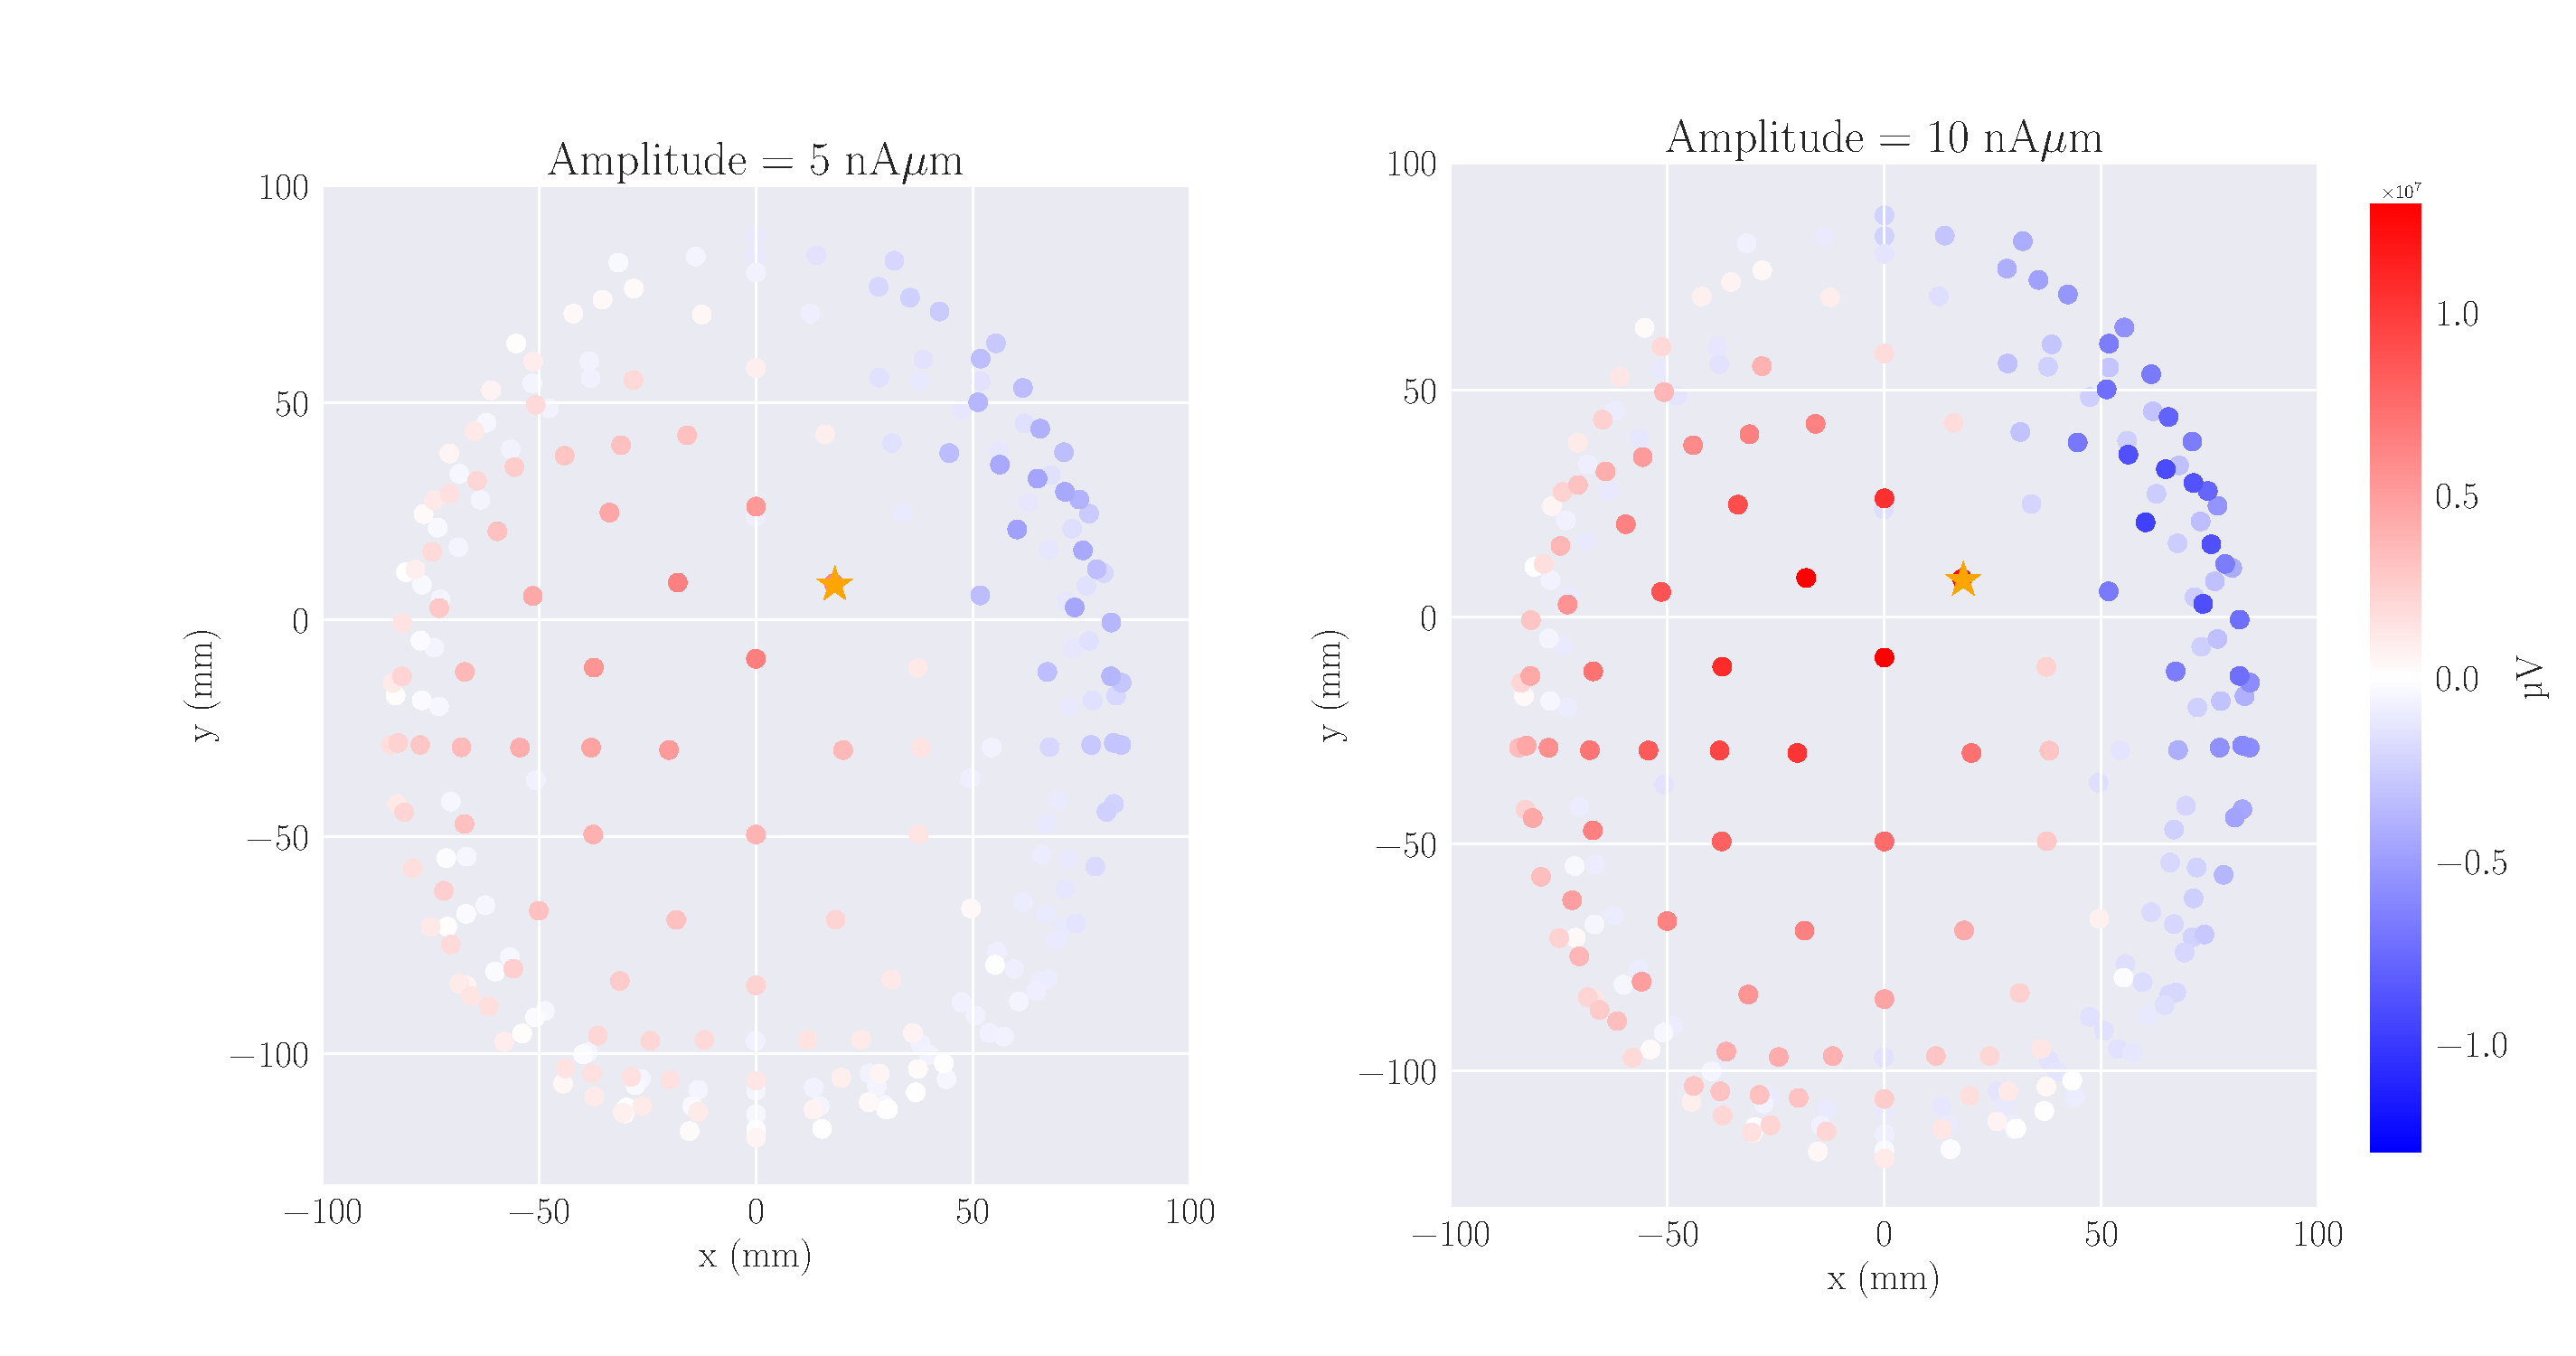
\includegraphics[width=\linewidth]{figures/dipole_w_amplitude_example.pdf}
    \caption{EEG data for two samples with current dipole amplitude equal to 5 and 10 nA$\mu$m. The EEG recordings have a range between -10 and 10 $\mu$V.}
    \label{fig:dipole_w_amplitude_example}
\end{figure}


\subsection{Performance Evaluation}
To assess the network's performance, we start by analyzing the accuracy in relation to training epochs, as depicted in Figure \ref{fig:dipole_w_amplitude_loss}. We emphasize that it is important to note that the target values have been normalized, resulting in a unitless loss measurements. Therefore, the figure provides a qualitative representation of the network's training progress rather than precise loss values. The plot clearly demonstrates a consistent pattern of decreasing loss as the number of epochs increases, indicating that the network effectively captures the underlying data patterns. Moreover, both the training and validation loss stabilize after approximately 1100 epochs, suggesting that the network has reached its optimal performance level. Each epoch takes about 20 seconds to finish, leaving us with a training time of roughly 8.5 hours in total.

\begin{figure}[!htb]
    \centering
    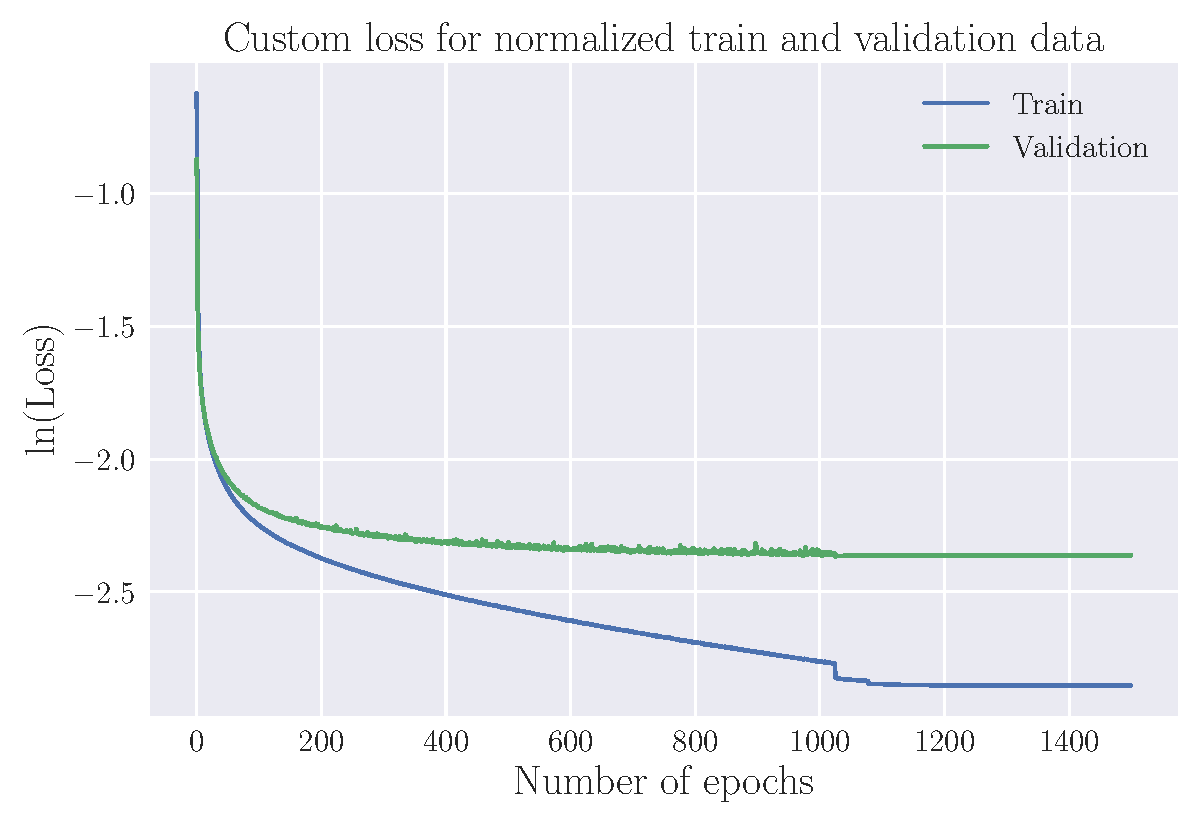
\includegraphics[width=\linewidth]{figures/NN_magnitude/Custom_Loss_amplitudes_test_custom_loss_tanh_32_0.001_0.35_0.1_0_1500_(0).pdf}
    \caption{Training and validation loss trends as functions of epochs for the DiLoc model, which predicts both location and magnitude parameters. The analysis is based on a dataset comprising 50,000 samples and spans a training duration of 1500 epochs.}
    \label{fig:dipole_w_amplitude_loss}
\end{figure}


In Figure \ref{fig:dipole_w_amplitude_targets}, we present the progression of the loss for the target parameters. Notably, after approximately 1100 epochs, all target values, exhibit a cessation of fluctuation, suggesting potential full convergence at this juncture. It is evident that the loss for the magnitude target converges significantly earlier in the training process, compared to the target coordinates, although at a notably higher numerical value. In contrast, the $x$, $y$, and $z$-coordinate targets display ongoing improvement until approximately 1100 epochs, gradually converging to values that closely align with one another. Among these, the $y$-coordinate achieves the lowest loss, followed by the $x$-coordinate, and then the z-coordinate.

\begin{figure}[!htb]
    \centering
    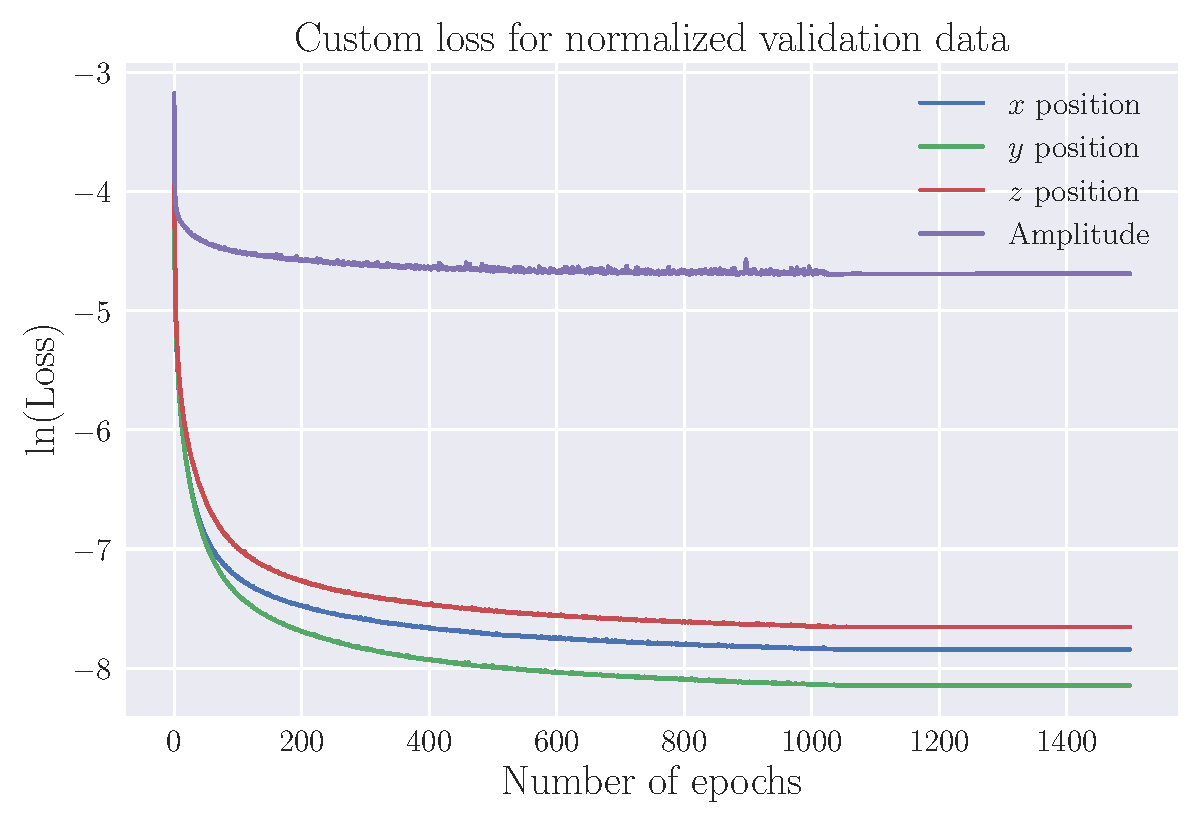
\includegraphics[width=\linewidth]{figures/NN_magnitude/Custom_Loss_mse_targets_amplitudes_test_custom_loss_tanh_32_0.001_0.35_0.1_0_1500_(0).pdf}
    \caption{Validation loss as a function of epoch for each target value, including the $x$, $y$, and $z$-coordinates of the dipole, as well as the magnitude of the dipole signal.}
    \label{fig:dipole_w_amplitude_targets}
\end{figure}


In Table \ref{table:error_simple_dipole}, we present the network's performance across various target categories using distinct error metrics. Analyzing the outcomes pertaining to the target coordinates reveals a noteworthy consistency in mean absolute error, with an average deviation of less than 1.5 mm from the true values. This level of accuracy is highly satisfactory. Considering the range associated with each coordinate profile, we observe that the MAE for the $x$ coordinate, at 1.348 mm, accounts for only 0.936$\%$ of the complete range. Similarly, for the $y$-coordinate, exhibiting a MAE of 1.448 mm, the error relative to the coordinate range stands at 0.809$\%$. Lastly, the $z$ coordinate, with a MAE of 1.411 mm, represents 1.052$\%$ of the full range. This balanced distribution of errors suggests that no single dimension to a large extent exhibits higher error propensity than the others, thereby indicating robust overall performance. It is important to note, however, that the $z$ coordinate consistently exhibits the largest error, implying that specific challenges or characteristics may exist in predicting this dimension, resulting in slightly elevated errors. Moving on to the MAE for the magnitude variable, we ascertain a value of 0.539 nA$\mu$m. In the context of a magnitude range spanning from 1 to 10 nA$\mu$m, this MAE translates to a relative error of 6.00$\%$, which is noticeably larger when compared to the MAE values for the target coordinates.

In addition to MAE, we look into the network's performance through the metrics of mean squared error and root mean squared error metrics, which offer complementary insights. For the $x$ coordinate, the MSE stands at 3.438 mm$^2$, while for the $y$- and $z$-coordinate, it is 3.860 mm$^2$ and 3.862 mm$^2$, respectively. MSE, due to its quadratic nature, penalizes larger errors more prominently. Despite this, the MSE values remain within reasonable bounds when contextualized within the coordinate ranges, implying a stable error profile with few significant outliers. Turning our attention to the MSE for the magnitude target, which measures 0.650 nA$^2\mu$m$^2$, we observe that it is lower than the MSE values for the coordinate targets. This is a satisfying finding, especially considering the narrower range of the magnitude target. However, it is important to recognize that the theoretical lower limit of MSE is always 0, which means there is still room for further improvement in accurately capturing variations in all the target values.

Lastly, the Root Mean Squared Error (RMSE), which indicates the standard deviation of prediction errors and their distribution around the mean, reports values slightly lower than the corresponding Mean Squared Error (MSE) values. Specifically, RMSE values measure at 1.854 mm, 1.965 mm, and 1.965 mm for the distinct target coordinates, and at 0.806 nA$\mu$m for the magnitude target. These RMSE values suggest that, on average, the prediction errors align with the overall spread of errors, without significant outliers or extreme deviations from the mean error. This indicates a level of stability and predictability in the error distribution.



\begin{table}[!htb]
\begin{tabular}{l|
>{\columncolor[HTML]{FFFFFF}}c
>{\columncolor[HTML]{FFFFFF}}c
>{\columncolor[HTML]{FFFFFF}}c
>{\columncolor[HTML]{FFFFFF}}c
>{\columncolor[HTML]{FFFFFF}}c |}
\cline{2-6}
                                                   & \multicolumn{5}{c|}{\cellcolor[HTML]{CBCEFB}\textbf{Error Metrics for Target Values}}                                                                                                                                                                                                                                                                                                                                                                                                                                                                                            \\ \cline{2-6}
                                                   & \multicolumn{1}{l|}{\cellcolor[HTML]{EFEFEF}\begin{tabular}[c]{@{}l@{}}x-coordinate\\ {[}mm{]}\end{tabular}} & \multicolumn{1}{l|}{\cellcolor[HTML]{EFEFEF}\begin{tabular}[c]{@{}l@{}}y-coordinate\\ {[}mm{]}\end{tabular}} & \multicolumn{1}{l|}{\cellcolor[HTML]{EFEFEF}\begin{tabular}[c]{@{}l@{}}z-coordinate\\ {[}mm{]}\end{tabular}} & \multicolumn{1}{l|}{\cellcolor[HTML]{EFEFEF}\begin{tabular}[c]{@{}l@{}}Position \\ Error {[}mm{]}\end{tabular}} & \multicolumn{1}{l|}{\cellcolor[HTML]{EFEFEF}\begin{tabular}[c]{@{}l@{}}Magnitude\\ {[}nA$\mu$m{]}\end{tabular}} \\ \hline
\multicolumn{1}{|l|}{\cellcolor[HTML]{EFEFEF}MAE}  & \multicolumn{1}{c|}{\cellcolor[HTML]{FFFFFF}1.348}                                                           & \multicolumn{1}{c|}{\cellcolor[HTML]{FFFFFF}1.448}                                                           & \multicolumn{1}{c|}{\cellcolor[HTML]{FFFFFF}1.420}                                                           & \multicolumn{1}{c|}{\cellcolor[HTML]{FFFFFF}1.405}                                                                  & 0.539                                                                                                           \\ \hline
\multicolumn{1}{|l|}{\cellcolor[HTML]{EFEFEF}MSE}  & \multicolumn{1}{c|}{\cellcolor[HTML]{FFFFFF}3.438}                                                          & \multicolumn{1}{c|}{\cellcolor[HTML]{FFFFFF}3.860}                                                          & \multicolumn{1}{c|}{\cellcolor[HTML]{FFFFFF}3.862}                                                          & \multicolumn{1}{c|}{\cellcolor[HTML]{FFFFFF}3.720}                                                                 & 0.650                                                                                                           \\ \hline
\multicolumn{1}{|l|}{\cellcolor[HTML]{EFEFEF}RMSE} & \multicolumn{1}{c|}{\cellcolor[HTML]{FFFFFF}1.854}                                                           & \multicolumn{1}{c|}{\cellcolor[HTML]{FFFFFF}1.965}                                                           & \multicolumn{1}{c|}{\cellcolor[HTML]{FFFFFF}1.965}                                                           & \multicolumn{1}{c|}{\cellcolor[HTML]{FFFFFF}1.929}                                                                  & 0.806                                                                                                           \\ \hline
\end{tabular}
\caption{\textbf{Evaluation of Diloc's performance utializing different Error Metrics.} \newline
Performance for the extended DiLoc network on test dataset consisting of 1000 samples. The errors are measured using Mean Squared Error (MSE), Mean Absolute Error (MAE), and Root Mean Squared Error (RMSE).}
\label{table:error_simple_dipole}
\end{table}

In Figure \ref{fig:magnitude_errors}, we present the MAE and MSE metrics computed between predicted and target coordinate values, as function of the magnitude of the dipole strengths. The figure reveals an interesting pattern, where the occurrence of outliers and less favorable predictions is higher when dealing with identification of dipoles with smaller magnitudes.

This apparent trend might initially suggest that the neural network encounters greater challenges in accurately predicting the posistions of dipoles with smaller magnitudes. However, we cannot rule out that these disparities might be related to alternative factors as depth positioning, intricate cortical folding patterns, or other random fluctuations. Nevertheless, the most pronounced trend that emerges from the figure is the prevalence of predictions exhibiting an AE smaller than 5 nA$\mu$m and a SE smaller than 10 nA$^2 \mu$m$^2$. This trend is of particular significance, serving as a reassuring indicator. It suggests that, despite observed variations in predictions for samples with smaller magnitudes, the majority of our Diloc’s predictions consistently cluster within a range with acceptable errors.

\begin{figure}
  \hspace*{-3cm} % Adjust the value as needed to move the figures left
  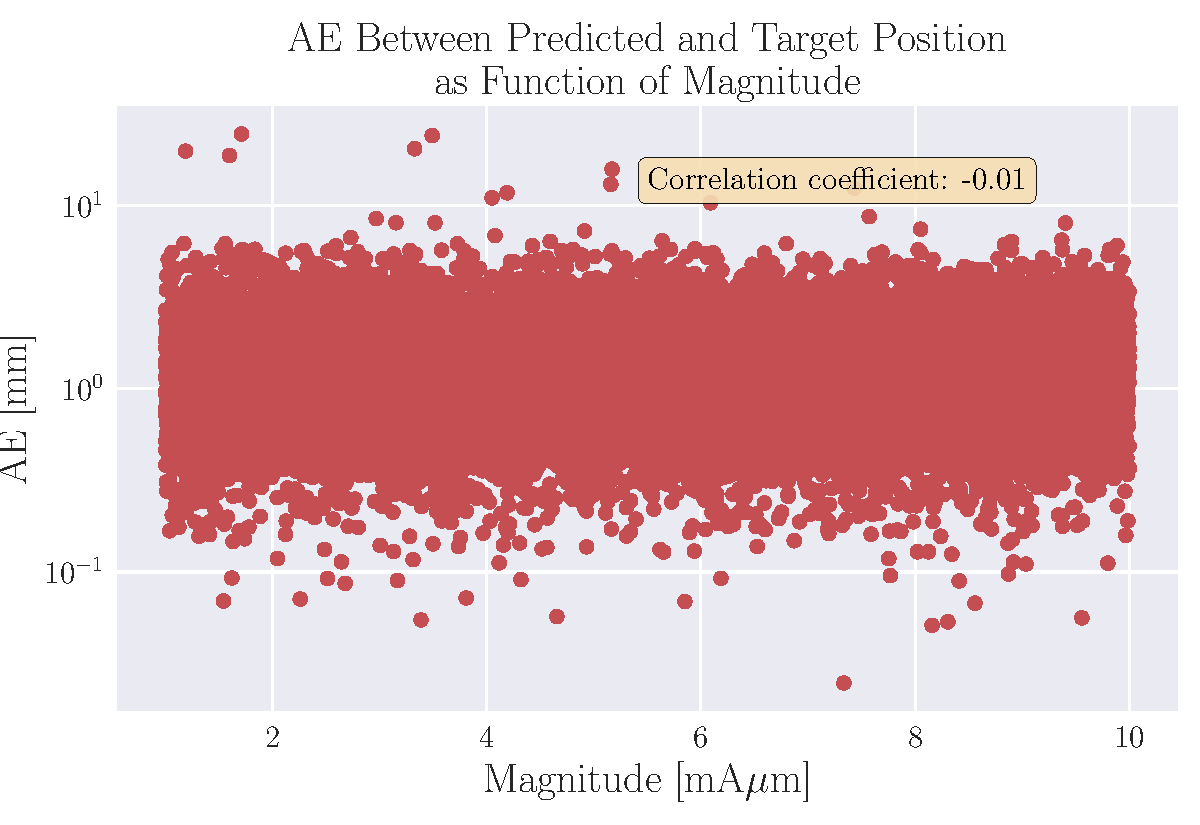
\includegraphics[width=9cm]{figures/NN_magnitude/mae_amplitude.pdf}
  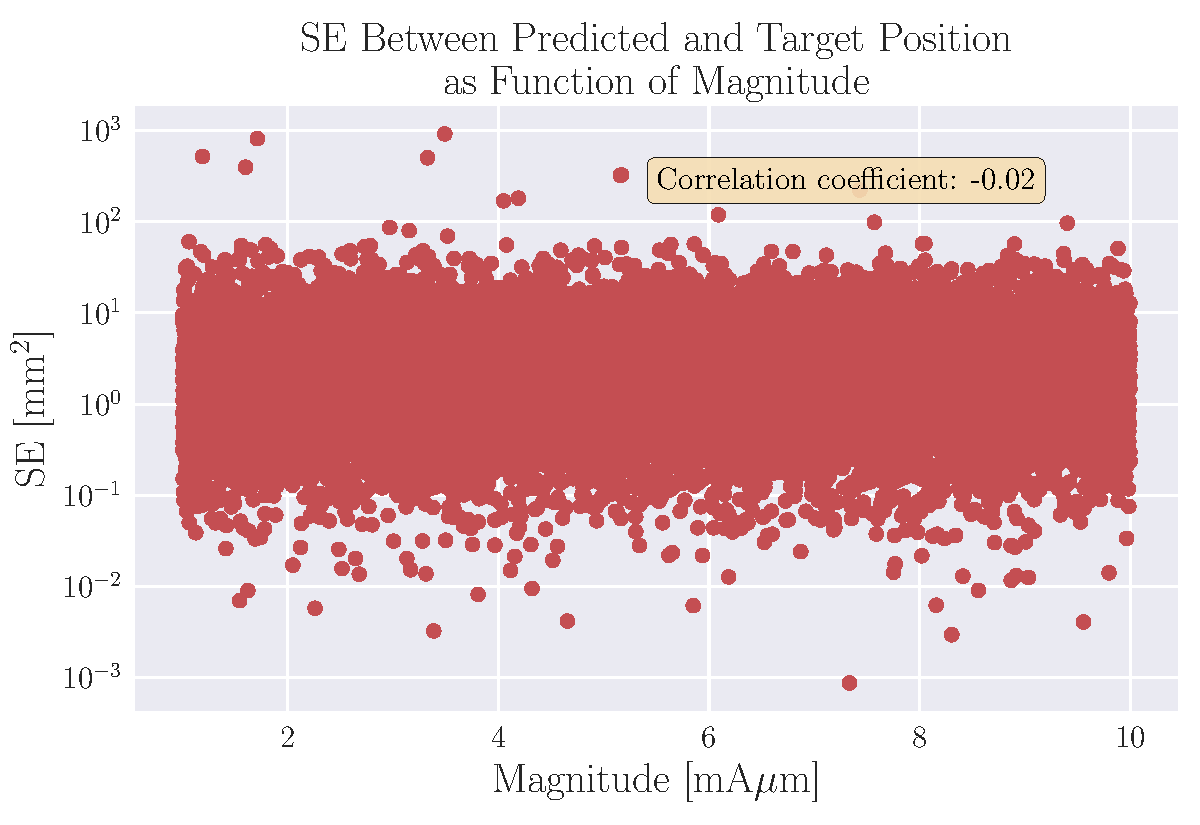
\includegraphics[width=9cm]{figures/NN_magnitude/mse_amplitude.pdf}
  \caption{Scatter plot of Abolsute Error and Squared Error computed between predicted and target coordinate values, as function of the magnitude of the dipole strengths.}
  \label{fig:magnitude_errors}
\end{figure}

The Mean Euclidean Distance (MED) of DiLoc's predictions on the unseen test data is measured at 2.815 mm. This represents a value more than 100$\%$ larger than the MED obtained when DiLoc predicted only the dipole locations for dipoles with a constant magnitude of electrical signal. Nevertheless, it is crucial to underscore that, given the dimensions of the brain within the NYHM, and the theshold value we aim to laty under, this error is relatively small and satisfactory.

Table \ref{table:MED_magnitude} presents the percentages of predictions of test samples falling within various MED threshold values. Notably, the network achieves an accuracy smaller than 12 mm for 99.8$\%$ of the test data. Furthermore, 64.3$\%$ of the samples exhibit a MED smaller than 3 mm, an achievement that, while robust, falls slightly short of DiLoc's performance in the previous, less complex problem.

\begin{table}[]
\begin{tabular}{|cccl|}
\hline
\rowcolor[HTML]{CBCEFB}
\multicolumn{4}{|c|}{\cellcolor[HTML]{CBCEFB}\textbf{Mean Euclidian Distance for Test Samples}}                                                                                                                                                                 \\ \hline
\rowcolor[HTML]{EFEFEF}
\multicolumn{1}{|c|}{\cellcolor[HTML]{EFEFEF}MED \textless 3 mm} & \multicolumn{1}{c|}{\cellcolor[HTML]{EFEFEF}MED \textless 5 mm} & \multicolumn{1}{c|}{\cellcolor[HTML]{EFEFEF}MED \textless 10 mm} & MED \textless 12 mm                                     \\ \hline
\rowcolor[HTML]{FFFFFF}
\multicolumn{1}{|c|}{\cellcolor[HTML]{FFFFFF}64.325 $\%$}        & \multicolumn{1}{c|}{\cellcolor[HTML]{FFFFFF}90.930 $\%$}        & \multicolumn{1}{c|}{\cellcolor[HTML]{FFFFFF}99.505 $\%$}         & \multicolumn{1}{c|}{\cellcolor[HTML]{FFFFFF}99.820 $\%$} \\ \hline
\end{tabular}
\caption{\textbf{MED evaluation on test samples; Predicting Location and Magnitude} \newline
Performance of the network on thes test dataset comprising 20,000 samples, presented as the percentage of samples falling within MED thresholds of 3 mm, 5 mm, 10 mm, and 12 mm, respectively.}
\label{table:MED_magnitude}
\end{table}



Figure \ref{fig:histogram_magnitude} displays two panels, depicting the MED and Mean Absolute Error (MAE) for the magnitude of each test sample within bins of width 1 unit. In the left panel, representing the MED histogram, the bins corresponding to MED values of 2 and 3 mm are the most populated, containing the largest proportion of samples. This panel also illustrates that the majority of predicted locations exhibit a MED error smaller than 14 mm, which is a satisfactory outcome.

Turning our attention to the right panel, which displays the MAE for predicted magnitudes, we observe that the bin holding samples with a magnitude prediction MAE less than 1 nA$\mu$m is the most populous. Within this bin, 17,014 out of the 20,000 samples fall, signifying that the network predicts the magnitude with a MED smaller than 1 nA$\mu$m for approximately 85$\%$ of the sample set.


\begin{figure}
  \hspace*{-2cm} % Adjust the value as needed to move the figures left
  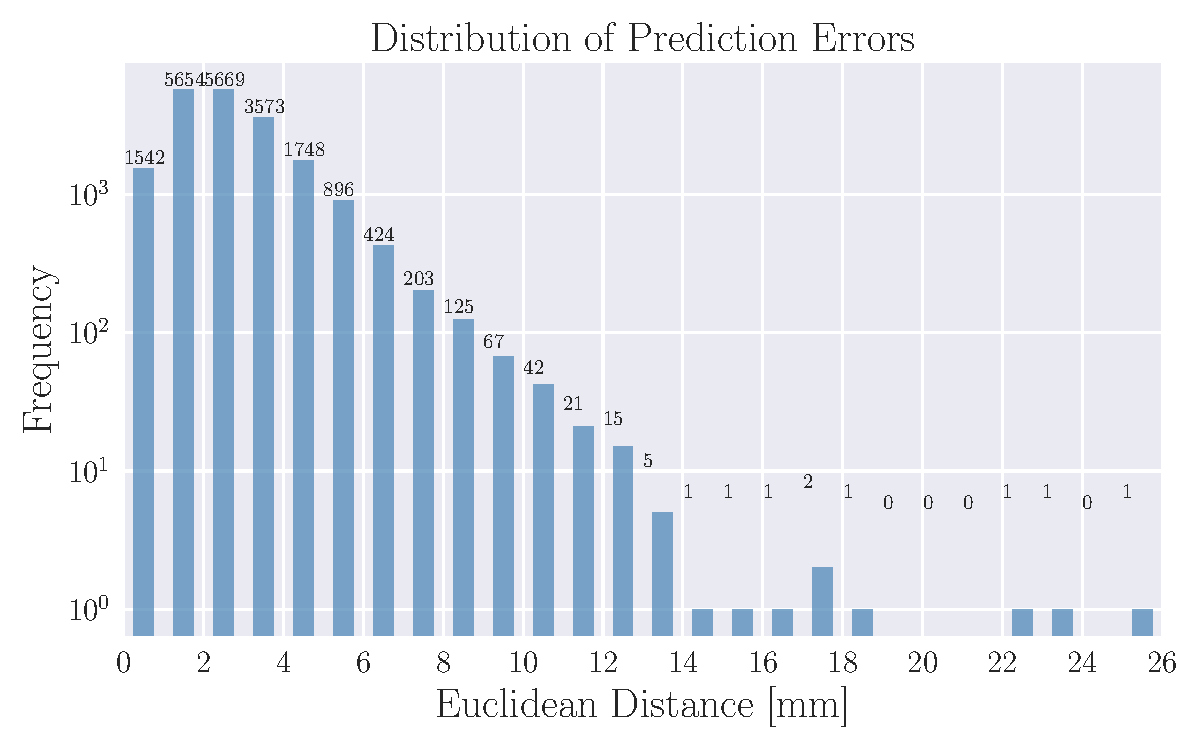
\includegraphics[width=9cm]{figures/new_histogram_position_amplitude.pdf}
  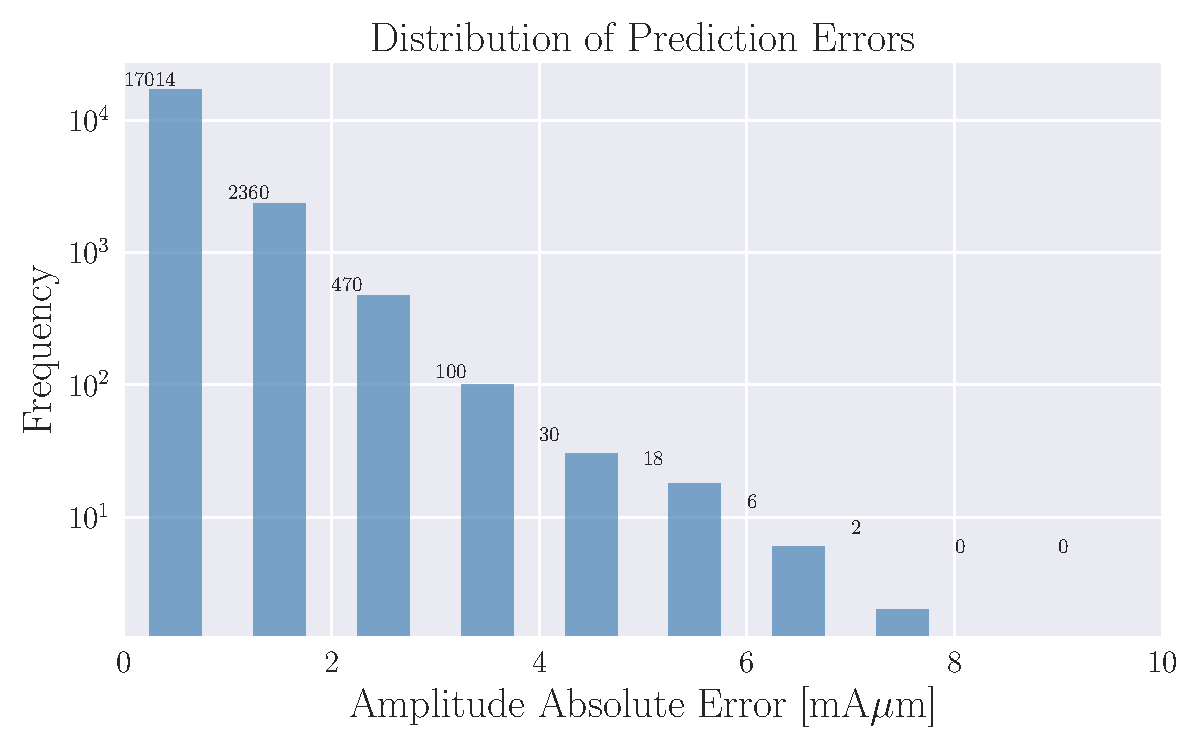
\includegraphics[width=9cm]{figures/new_histogram_amplitude_amplitude.pdf}
  \caption{Left panel illustrates the distribution of Mean Euclidean Distance for the predicted dipole locations, organized into bins of width 1 mm. Right panel holds the distribution of Mean Absolute Error for the predicted magnitude of dipole electrical signal, presented in a similar format, with bins of width 1 nA$\mu$m.}
  \label{fig:histogram_magnitude}
\end{figure}










\section{Predicting Region of Active Correlated Current Dipoles with Magnitudes}

In order to further enhance the complexity of our problem, we extend the DiLoc neural network to incorporate varying radii and magnitudes for the origins generating the electrical activity detected by the recording electrodes. This transformation alters the objective of the DiLoc network from predicting the location of individual current dipole moments to estimating the centers of larger spherical populations. This extension is hopefully valuable for real-life scenarios where understanding the extent of brain abnormalities causing unusual activity in affected areas may be of interest. By training the DiLoc network on such complex data, we aim to enhance its ability to generalize and perform effectively in real-world clinical cases

\subsection{Adjusting Data Set}
\rednote{Include that with this arcitecture the amplitude/radius is more weighted than position since correlation between magnitude and radius. }
\rednote{Also include wd value}

In order to optimize the neural network's capacity for predicting dipole population regions, we made specific adjustments to the dataset. Within this framework, each dipole population comprises individual dipoles distributed across all points within the NY head cortex falling within a spherical volume ranging from 1 mm to 15 mm in radius. Notably, guidelines established by Delucchi et al. (1962), Cooper et al. (1965), Ebersole (1997), Nunez and Srinivasan (2006), and Schomer and Lopes da Silva (2018) in the clinical context of spontaneous EEG, suggest that for EEG recordings to detect brain activity, approximately 6-10 cm$^2$ of contiguous brain tissue must exhibit synchronous activity. A spherical radius of 15 mm translates to an approximate area of 7 cm$^2$, and thus falls within this criterion.

However, it is important to acknowledge that when we shift our focus to EEG data derived from scalp recordings averaged over multiple trials,  particularly in event-related potentials (ERP) experiments, a different perspective also emerges from their work. In ERP studies, researchers primarily investigate the brain's responses to specific stimuli. To enhance the reliability of these responses, trial-averaging is a common practice. Consequently, as suggested by these authors, it becomes plausible that EEG activity arising from brain regions smaller than the typical 6-10 cm$^2$ criterion for spontaneous EEG could be detectable under such circumstances. This observation gains significance when considering the potential detection of brain activity within smaller regions, particularly when trial-averaging is employed, thereby enabling the identification of neural populations smaller than the conventional 6 cm$^2$ threshold.


For simplification reasons, we wanted to maintain the maximum amplitude strength of the total populations at 10 mA$\mu$m. Consequently, we had to calculate the maximum number of points within a volume sphere with a radius of 15 mm and reduce this number by 10 in order to determine the strength of a distinct dipole within a given area. Having that the maximum number of dipoles that fit within a volume sphere with an ideal center and radius 15 mm was 899 dipoles, we were left with a dipole strength of 10/899 for each dipole. The strength of a dipole population is thus directly proportional to the size of the dipole population. While this may not perfectly represent real-world scenarios, it provides a reasonable approximation for our model.


In Figure \ref{fig:dipole_area}, we present an example of a dipole population and the corresponding EEG signal. The upper panels show the EEG signals for the specific sample, seen from different angels. The recording electrode locations are presented as filled circles, where the color of the fill represents the amplitude of the measured EEG signal for the given electrode. The yellow filled circles in the plots in the lower panel represents the diple populations, i.e. positions within the cortex where dipoles have been placed. The plots within the figure are seen from the x-z plane, x-y plane, and y-z plane.

\begin{figure}[!htb]
\centering
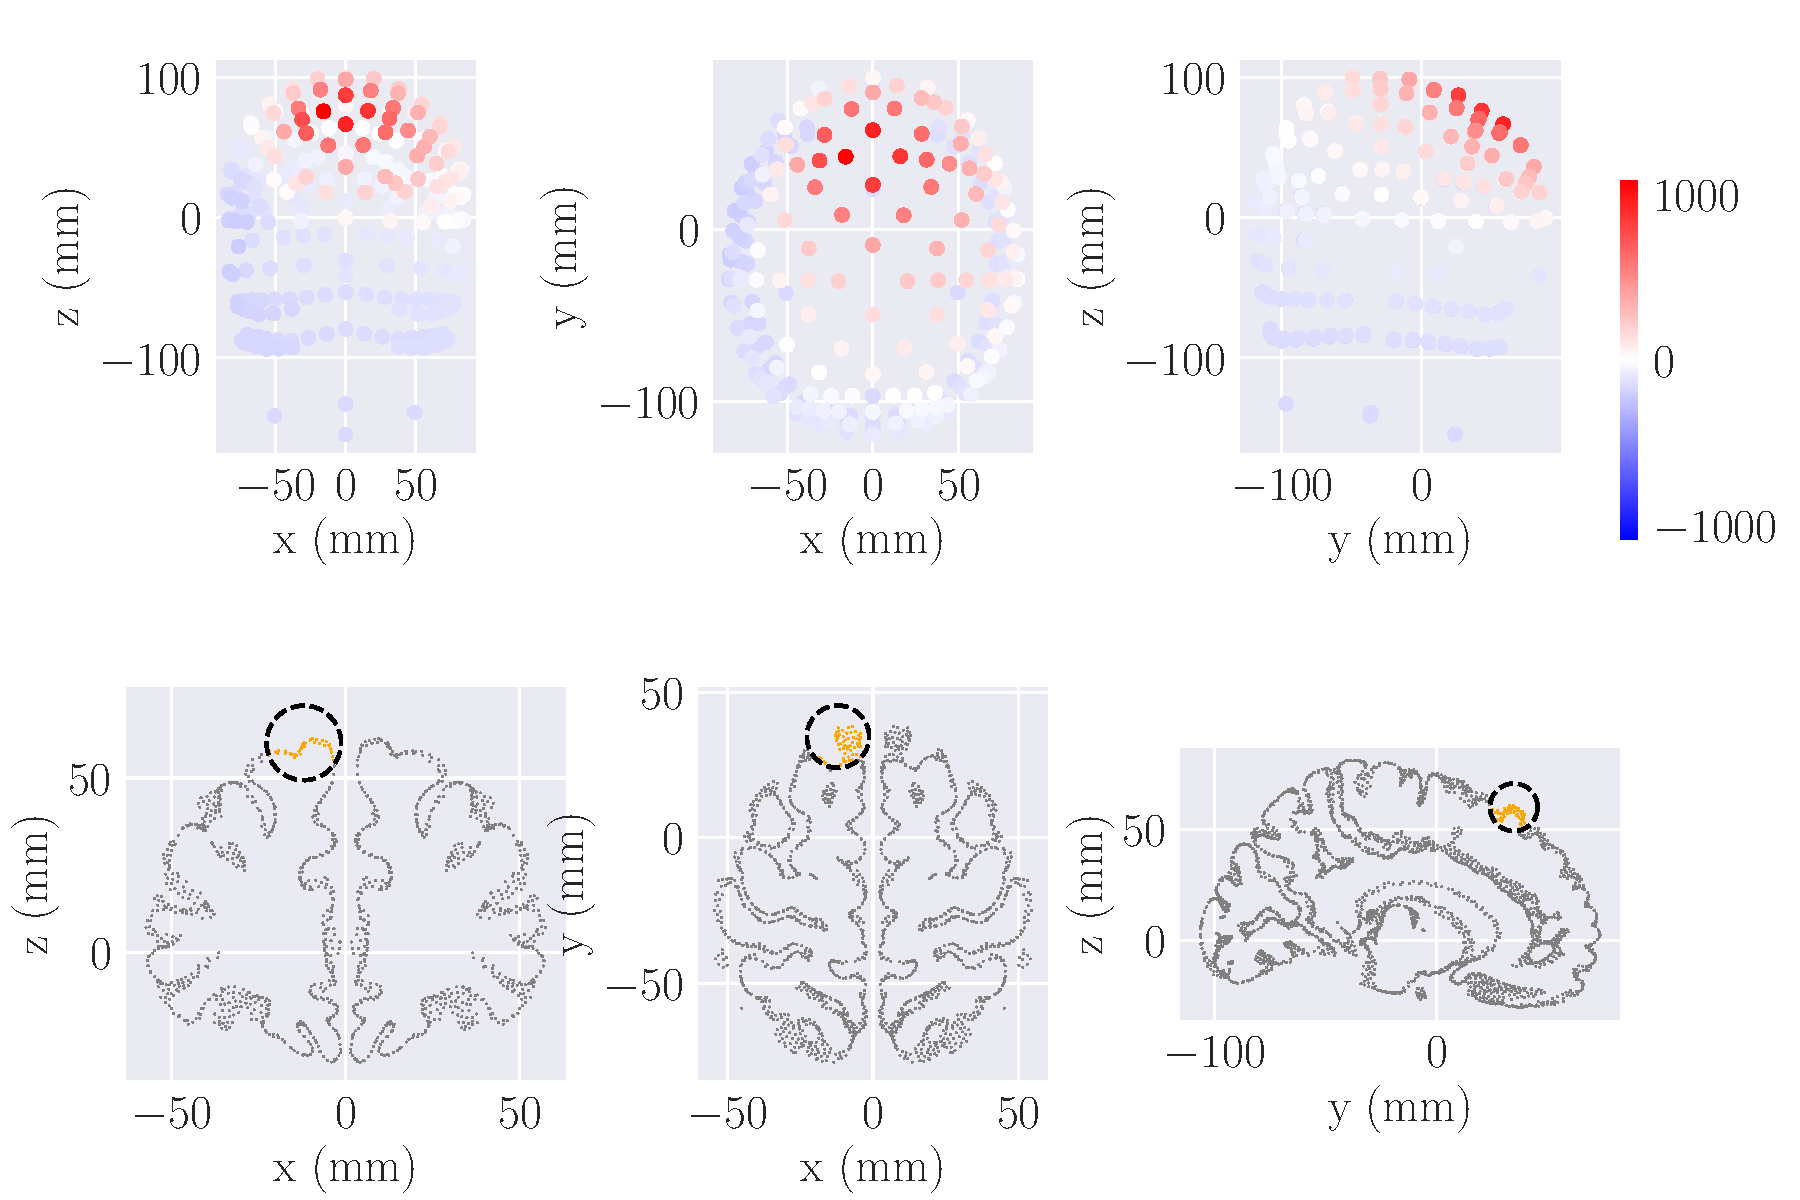
\includegraphics[width=\linewidth]{figures/dipole_area_reduced_0.pdf}
\caption{EEG for a sample containing a spherical population of current dipole sources with a random center within the cerebral cortex.
\textbf{Upper panels:}
The EEG measure is seen from the front (x-z plane), side (y-z plane), and top (x-y plane) of the cortex. EEG electrode locations are presented as filled circles, where the color of the fill represents the amplitude of the measured signal for the given electrode.
\textbf{Lower panels:}
Gray filled circles represent points within the NY cortex where a dipole could have been placed. Yellow filled circles represent positions within the cortex where dipoles have been placed.}
\label{fig:dipole_area}
\end{figure}

% \rednote{Place somewhere else if needed?}
% As for the dataset, the number of target values is now 5: x, y, z-coordinates of the center of the dipole population, total magnitude, and radius. The number of features within the dataset is not modified and still holds 231 values, representing the EEG signal measured at every recording electrode.

% \begin{figure}[!htb]
% \centering
% 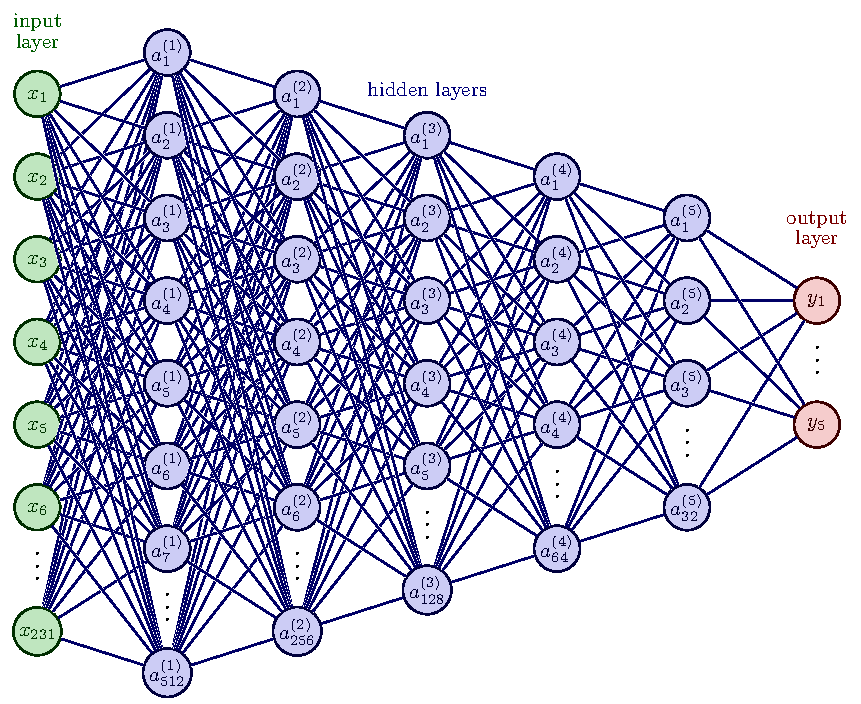
\includegraphics[width=\linewidth]{figures/NN_dipole_area_architecture.pdf}
% \caption{Architecture of the dipole area prediction network.}
% \label{fig:NN_dipole_area_architecture}
% \end{figure}

% \rednote{Rewrite/remove}
% Similar to the previous problem, we normalize the target values to ensure they all range from 0 to 1. Moreover, in this extension of the DiLoc network, we use the same activation functions as in the previous problem with ReLU as the activation function in the first layer, hyperbolic tangent for the hidden layers, and the Sigmoid activation function in the output layer.
%As with the previous problems, we have explored various network architectures and activation functions, but the current configuration has shown the best performance in terms of accurate predictions for this problem. It is important to emphasize that our primary goal is to find a network that can effectively solve the problem and provide accurate predictions, rather than necessarily seeking the best possible configuration.


\subsection{Performance Evaluation}
% How does the loss relate to size of population
% Exammple run and how long time it takes to calculate

In Figure \ref{fig:dipoile_area_result}, we present the training and validation costumized loss for the DiLoc network as a function of epochs. We once again emphasize that since the network's loss is unitless, meaning that the figure only provides a visual representation of the network's training progress rather than directly interpretable loss values. The network was trained for 1000 epochs. We se a clear trend of decreasing loss with an increasing number of epochs. However, after epoch 800, there both train and validation loss seem to have reach convegence, and no further improvement in loss shows. We can therefor conclude that overfitting has not taken place during training. At epoch 749, the learning rate is adjusted from 0.001 to 0.00004, to which we can observe a dip in the loss, and the ending of fluctuastions/ stochasticity in the validation loss. On average, each epoch uses 23 seconds to fininsh, leading to a fully training time of roughly 9.5 hours.


\begin{figure}[!htb]
    \centering
    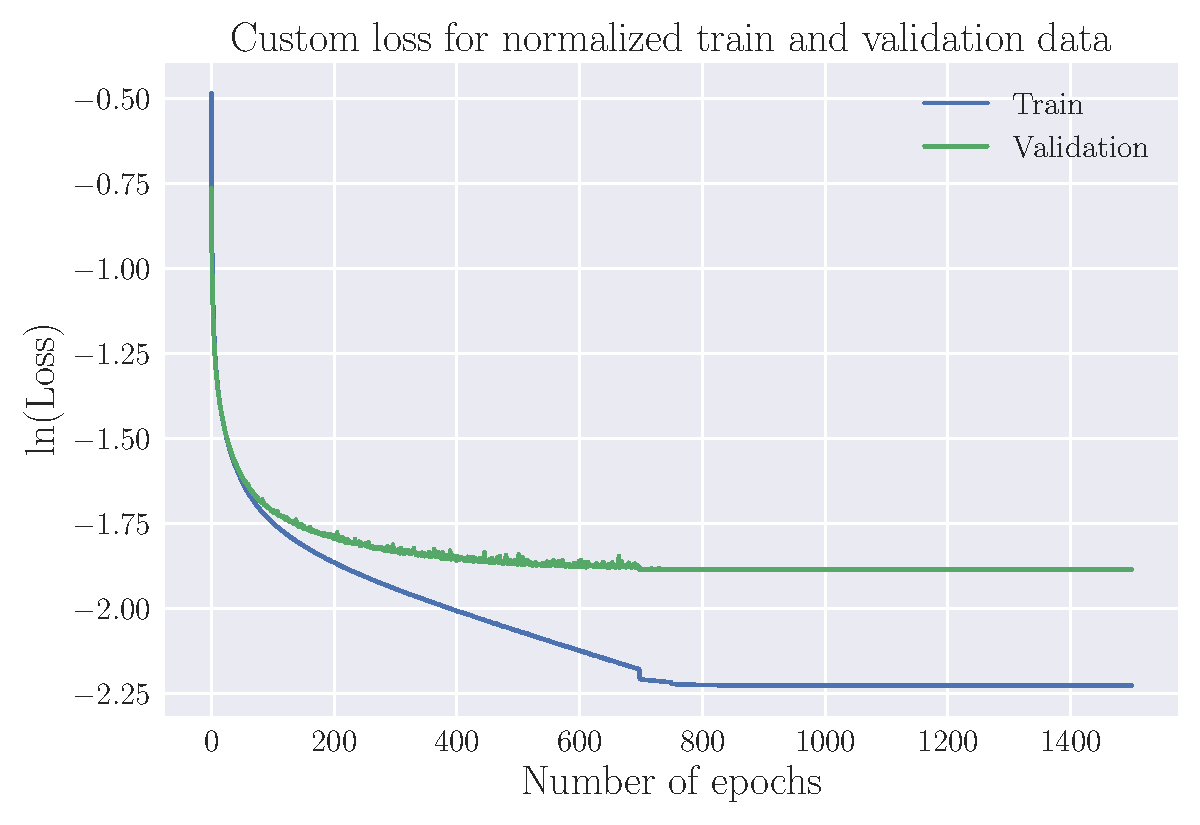
\includegraphics[width=\linewidth]{figures/NN_area/Custom_Loss_area_seed_42_cnn_32_0.001_0.35_0.1_0_1500_(0).pdf}
    \caption{Training and validation custom loss trends as functions of epochs for the DiLoc model, which predicts both the center and radius parameters. The analysis is based on a dataset comprising 50,000 samples and spans a training duration of 1500 epochs.}
    \label{fig:dipole_area_result}
\end{figure}

Figure \ref{fig:dipole_area_target_result} displays the validation loss for each target value as a function of epochs. We observe that the loss for all target coordinates are smallest as approximately 100, and from here has an observable increase, before stabilazing at approximatly 800 epochs. Here the MSE loss for the $x-$ and $z-$ coordinates are somewhat alike and stabilizes at a larger loss than the one corresponding to the $y$- coordinate. Shifting our focus to the magnitude and radius targets, we observe that the loss evaluations corresponding to these vales look much the same. The loss curves "follow" each other, however the radius loss curve is higher than the magnitude loss. Somewhere between 700 and 800 epochs these lkoss curves also converges. Even thogh loss corresponding to the target coordinates has its lowest loss values at an ealier stage, the model aim to minimize the total loss, and therefor the training cannot stop where the loss of the coordinates has its minima.

\begin{figure}[!htb]
    \centering
    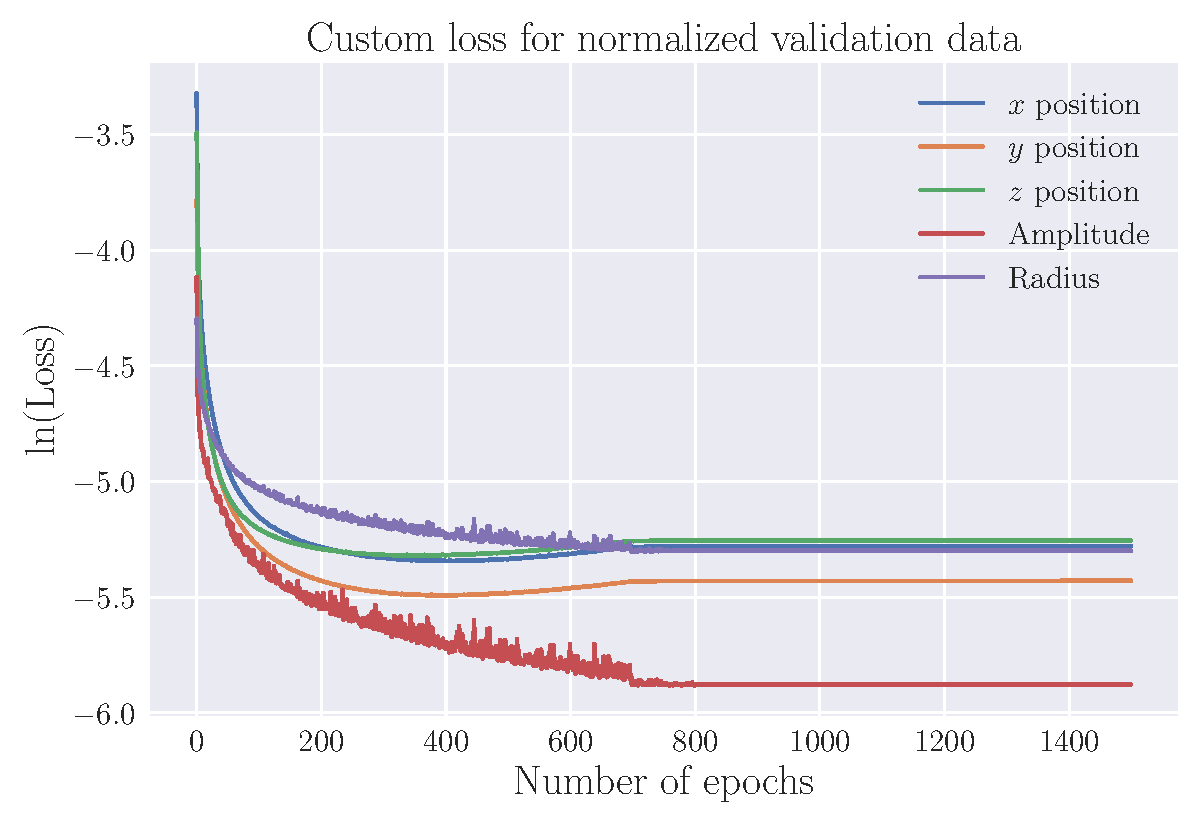
\includegraphics[width=\linewidth]{figures/NN_area/Custom_Loss_mse_targets_area_seed_42_cnn_32_0.001_0.35_0.1_0_1500_(0).pdf}
    \caption{Validation MSE loss as a function of epoch for each target value, including the $x$, $y$, and $z$-coordinates of the center of the dipole population, as well as the amplitude and radius.}
    \label{fig:dipole_area_target_result}
\end{figure}

\FloatBarrier


We furter evaluate our model predictions, by feeding it with the unseen test data set, and by denormalize the output of the network and comparing it to the target values the MED between the predicted and target coordinates measures to 7.85 mm, MAE between predicted and target magnitude equals 0.33 mA$\mu$m and MAE between predicted and target radius is 0.76 mm. The MED measures a slightly higher value compared to when predicting only position and magnitude strenght of the dipole. However, we note that the MAE corresponding to the magnitude has decreased in this more complex problem, now corresponding to a relative error of only 3.67$\%$. In table \ref{tab:Loss_dipole_area} we can read off the percentages of the network predictions of test samples that falls within various threshold values. We have that 79.68 $\%$ of the predictions has a ED in position smaller than 10 mm, 98.57$\%$ an AE in magnitude smaller than 2 mA$\mu$m and 97.22$\%$ an AE in radius smaller than 3 mm.

Table \ref{tab:thresholds_dipole_area} further provides an overview of the percentage of samples than fulfill multiple of threshold values at once. These numbers has been found with the initial condition that all predictions fulfill the constraint that the ED between predicted and target position is smaller than 10 mm. A result drawn from the table is that 78.290$\%$ of DiLoc'section predictions has an AE smaller than 2 mA$\mu$m in magnitude and $3$ mm in radius.


\begin{table}[]
\hspace*{-4cm}
\begin{tabular}{|ccc|l|ccc|l|ccc|}
\cline{1-3} \cline{5-7} \cline{9-11}
\multicolumn{3}{|c|}{\cellcolor[HTML]{CBCEFB}\textbf{Eucledian Distance: Position}}                                                                                                                                                                                                                             & \textbf{}             & \multicolumn{3}{c|}{\cellcolor[HTML]{CBCEFB}\textbf{Absolute Error: Magnitude}}                                                                                                                                                                                                                             & \textbf{}             & \multicolumn{3}{c|}{\cellcolor[HTML]{CBCEFB}\textbf{Absolute Error: Radius}}                                                                                                                                                                                                                                   \\ \cline{1-3} \cline{5-7} \cline{9-11}
\multicolumn{1}{|c|}{\cellcolor[HTML]{EFEFEF}\begin{tabular}[c]{@{}c@{}}ED \\ \textless 5 mm\end{tabular}} & \multicolumn{1}{c|}{\cellcolor[HTML]{EFEFEF}\begin{tabular}[c]{@{}c@{}}ED \\ \textless 10 mm\end{tabular}} & \cellcolor[HTML]{EFEFEF}\begin{tabular}[c]{@{}c@{}}ED \\ \textless 15 mm\end{tabular} &                       & \multicolumn{1}{c|}{\cellcolor[HTML]{EFEFEF}\begin{tabular}[c]{@{}c@{}}AE \\ \textless 1 mA$\mu$m\end{tabular}} & \multicolumn{1}{c|}{\cellcolor[HTML]{EFEFEF}\begin{tabular}[c]{@{}c@{}}AE\\ \textless 2 mA$\mu$m\end{tabular}} & \cellcolor[HTML]{EFEFEF}\begin{tabular}[c]{@{}c@{}}AE \\ \textless 3 mA$\mu$m\end{tabular} &                       & \multicolumn{1}{c|}{\cellcolor[HTML]{EFEFEF}\begin{tabular}[c]{@{}c@{}}AE \\ \textless 1 mm\end{tabular}} & \multicolumn{1}{c|}{\cellcolor[HTML]{EFEFEF}\begin{tabular}[c]{@{}c@{}}AE \\ \textless 3 mm\end{tabular}} & \cellcolor[HTML]{EFEFEF}\begin{tabular}[c]{@{}c@{}}AE \\ \textless 5 mm\end{tabular} \\ \cline{1-3} \cline{5-7} \cline{9-11}
\multicolumn{1}{|c|}{56.045$\%$}                                                                           & \multicolumn{1}{c|}{79.680$\%$}                                                                            & 86.435$\%$                                                                            & \multicolumn{1}{c|}{} & \multicolumn{1}{c|}{92.900$\%$}                                                                           & \multicolumn{1}{c|}{98.565$\%$}                                                                          & 99.685$\%$                                                                           & \multicolumn{1}{c|}{} & \multicolumn{1}{c|}{74.210$\%$}                                                                           & \multicolumn{1}{c|}{98.220$\%$}                                                                            & 99.770$\%$                                                                            \\ \cline{1-3} \cline{5-7} \cline{9-11}
\end{tabular}
\caption{}
\label{table:Loss_dipole_area}
\end{table}

\begin{table}[]
\begin{tabular}{l|ccc|}
\cline{2-4}
& \multicolumn{3}{c|}{\cellcolor[HTML]{CBCEFB}\textbf{\begin{tabular}[c]{@{}c@{}}Predictions within different thresholds\\ (Initial condition for position: ED \textless 10 mm)\end{tabular}}} \\ \cline{2-4}
& \multicolumn{1}{l|}{\cellcolor[HTML]{EFEFEF}AE \textless 1 mA$\mu$m} & \multicolumn{1}{l|}{\cellcolor[HTML]{EFEFEF}AE \textless 2 mA$\mu$m} & \multicolumn{1}{l|}{\cellcolor[HTML]{EFEFEF}AE \textless 3 mA$\mu$m} \\ \hline
\multicolumn{1}{|l|}{\cellcolor[HTML]{EFEFEF}AE \textless 1 mm} & \multicolumn{1}{c|}{58.075 $\%$} & \multicolumn{1}{c|}{59.940 $\%$} & 60.055 $\%$ \\ \hline
\multicolumn{1}{|l|}{\cellcolor[HTML]{EFEFEF}AE \textless 3 mm} & \multicolumn{1}{c|}{74.045 $\%$} & \multicolumn{1}{c|}{78.290 $\%$} & 78.765 $\%$ \\ \hline
\multicolumn{1}{|l|}{\cellcolor[HTML]{EFEFEF}AE \textless 5 mm} & \multicolumn{1}{c|}{74.315 $\%$} & \multicolumn{1}{c|}{78.890 $\%$} & 79.515 $\%$ \\ \hline
\end{tabular}
\caption{\textbf{Evaluation of DiLoc utilizing different Error Metrics.}
Performance of the extended DiLoc network on a test dataset consisting of 20000 samples. The errors are measured using Mean Absolute Error (MAE), Mean Absolute Percentage Error (MAPE), Mean Squared Error (MSE), and Root Mean Squared Error (RMSE) for various target values.}
\label{table:thresholds_dipole_area}
\end{table}



Once again, to make the accuracy of the model comparably to work done by others, and further assess the extent to which the network can predict the center of the dipole populations, in addition to amplitude and radius, we utilize the same evaluation metrics as done for the earlier problems: MAE, MSE ans RMSE. Table \ref{table:error_dipole_area} presents the Mean Absolute Error (MAE), Mean Squared Error (MSE), and Root Mean Squared Error (RMSE) for the predictions of the different sets of target parameters.

The MAEs for the target coordinates, i.e, center of the dipole population averages to 3.96 mm. This is the highest MAE measured for the predictions done by the netowrk when comparing all problems studied. An intersting observation however, is that in contrast to the other problems studied, the $z$-coordinate stands for the highest contribtuion to this MAE. This might therefor indicate that which coordinate DiLoc trobles the most with, is not necessary significant, but rather comes from randomness.

Regarding the MSE, we observe relatively small errors for the amplitude and radius, with values of 0.312 and 1.114 (mm$^2$) respectively. However, as for the target coordinate values, we encounter the highest observed MSE values so far. The MSE between the predicted and target coordinates ranges from 42.58 mm$^2$ and 66.816$^m$, suggesting the broadest dispersion of errors observed so far. The increase in RMSE is also apparent. This therefor suggest that, on average, the prediction errors does not always align with the overall spread of errors, meaning that the model sometimes will give accurate predictions and in other cases not so much. This therefor indicates a lower level of stability and predictability in the error distribution, compared to the other problems studied.

\begin{table}
\begin{tabular}{c|
>{\columncolor[HTML]{FFFFFF}}c
>{\columncolor[HTML]{FFFFFF}}c
>{\columncolor[HTML]{FFFFFF}}c
>{\columncolor[HTML]{FFFFFF}}c
>{\columncolor[HTML]{FFFFFF}}c
>{\columncolor[HTML]{FFFFFF}}c |}
\cline{2-7}
\multicolumn{1}{l|}{} & \multicolumn{6}{c|}{\cellcolor[HTML]{CBCEFB}\textbf{Error for different target values}} \\ \cline{2-7}
\multicolumn{1}{l|}{} & \multicolumn{1}{c|}{\cellcolor[HTML]{EFEFEF}\begin{tabular}[c]{@{}c@{}}x \\ {[}mm{]}\end{tabular}} & \multicolumn{1}{c|}{\cellcolor[HTML]{EFEFEF}\begin{tabular}[c]{@{}c@{}}y \\ {[}mm{]}\end{tabular}} & \multicolumn{1}{c|}{\cellcolor[HTML]{EFEFEF}\begin{tabular}[c]{@{}c@{}}z \\ {[}mm{]}\end{tabular}} & \multicolumn{1}{l|}{\cellcolor[HTML]{EFEFEF}\begin{tabular}[c]{@{}l@{}}Center \\ {[}mm{]}\end{tabular}} & \multicolumn{1}{l|}{\cellcolor[HTML]{EFEFEF}\begin{tabular}[c]{@{}l@{}}Magnitude \\ {[}nA$\mu$m{]}\end{tabular}} & \multicolumn{1}{l|}{\cellcolor[HTML]{EFEFEF}\begin{tabular}[c]{@{}l@{}}Radius \\ {[}mm{]}\end{tabular}} \\ \hline
\multicolumn{1}{|c|}{\cellcolor[HTML]{EFEFEF}MAE} & \multicolumn{1}{c|}{\cellcolor[HTML]{FFFFFF}3.819} & \multicolumn{1}{c|}{\cellcolor[HTML]{FFFFFF}4.342} & \multicolumn{1}{c|}{\cellcolor[HTML]{FFFFFF}3.722} & \multicolumn{1}{c|}{\cellcolor[HTML]{FFFFFF}3.961} & \multicolumn{1}{c|}{\cellcolor[HTML]{FFFFFF}0.325} & 0.765 \\ \hline
\multicolumn{1}{|c|}{\cellcolor[HTML]{EFEFEF}MSE} & \multicolumn{1}{c|}{\cellcolor[HTML]{FFFFFF}42.581} & \multicolumn{1}{c|}{\cellcolor[HTML]{FFFFFF}66.816} & \multicolumn{1}{c|}{\cellcolor[HTML]{FFFFFF}41.681} & \multicolumn{1}{c|}{\cellcolor[HTML]{FFFFFF}50.359} & \multicolumn{1}{c|}{\cellcolor[HTML]{FFFFFF}0.313} & 1.114 \\ \hline
\multicolumn{1}{|c|}{\cellcolor[HTML]{EFEFEF}RMSE} & \multicolumn{1}{c|}{\cellcolor[HTML]{FFFFFF}6.525} & \multicolumn{1}{c|}{\cellcolor[HTML]{FFFFFF}8.174} & \multicolumn{1}{c|}{\cellcolor[HTML]{FFFFFF}6.456} & \multicolumn{1}{c|}{\cellcolor[HTML]{FFFFFF}7.096} & \multicolumn{1}{c|}{\cellcolor[HTML]{FFFFFF}0.559} & 1.056 \\ \hline
\end{tabular}
\caption{\textbf{Dipole Population: Evaluation of DiLoc utilizing different Error Metrics.}
Performance of the extended DiLoc network on a test dataset consisting of 20,000 samples. The errors are measured using Mean Absolute Error (MAE), Mean Squared Error (MSE), and Root Mean Squared Error (RMSE) for various target values.}
\label{table:error_dipole_area}
\end{table}

In Figure \ref{fig:area_errors}, we present the MAE and MSE metrics computed between predicted and target magnitude values, as a function of the magnitude of the dipole strengths. The figure reveals an interesting pattern, where the occurrence of outliers and less favorable predictions is higher when dealing with identification of dipoles with smaller magnitudes.

This apparent trend might initially suggest that the neural network encounters greater challenges in accurately predicting smaller magnitudes. However, we cannot rule out that these disparities might be related to alternative factorsdepth positioning, intricate cortical folding patterns, or other random fluctuations. Nevertheless, the most pronounced trend that emerges from the figure is the prevalence of predictions exhibiting a MAE smaller than 5 nA$\mu$m and a MSE smaller than 10 nA$^2 \mu$m$^2$. This trend is of particular significance, serving as a reassuring indicator. It suggests that, despite observed variations in predictions for samples with smaller magnitudes, the majority of our Diloc’s predictions consistently cluster within a range with acceptable errors.

\begin{figure}
  \hspace*{-3cm} % Adjust the value as needed to move the figures left
  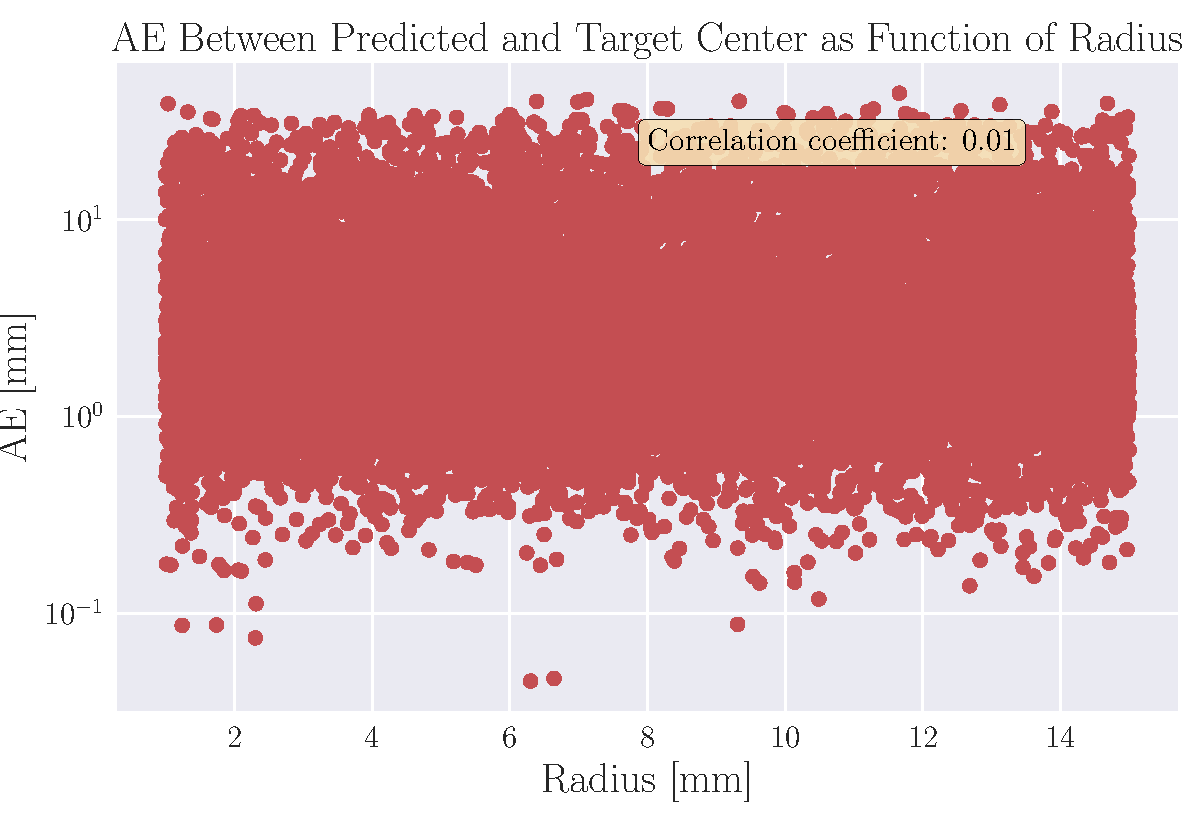
\includegraphics[width=9cm]{figures/NN_area/mae_area.pdf}
  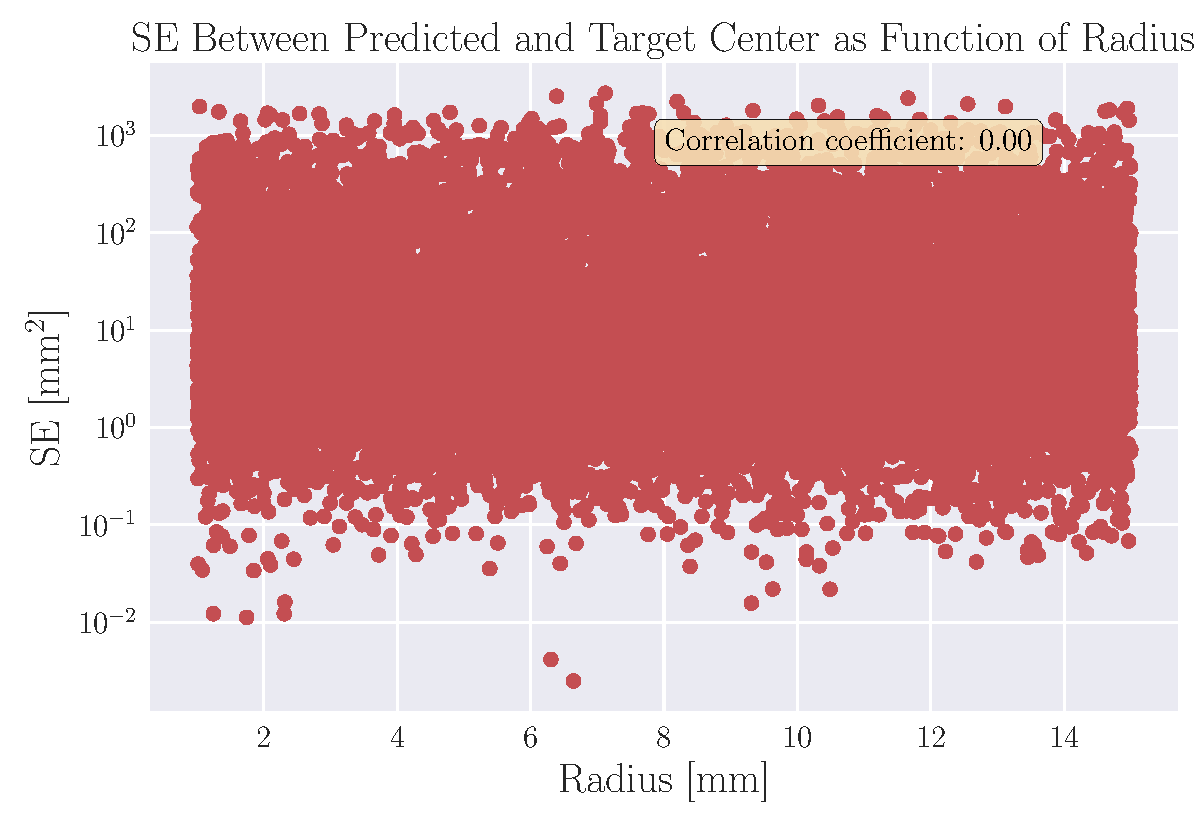
\includegraphics[width=9cm]{figures/NN_area/mse_area.pdf}
  \caption{\textbf{Dipole Population:}
  Scatter plot of Mean Abolsute Error and Mean Squared Error computed between predicted and target center values, as function of the radius of the dipole populations.}
  \label{fig:area_errors}
\end{figure}


\end{document}
